\documentclass[a4paper,12pt,oneside,openright]{book}
\usepackage[italian,english]{babel}
\usepackage[utf8]{inputenc} % inputenc serve a definire con che encoding stai realizzando il tuo documento .tex (quindi dipende dal fatto che tu stia usando Linux, Windows, Apple, o altro
\usepackage[T1]{fontenc} % fontenc definisce che tipo di caratteri utilizzare nel tuo output (pdf e dvi).

\usepackage{graphicx}
\usepackage{subfigure}
% senza uno di questi package dà errore sulla T nell'indice se lo compilo con Overleaf mentre è chiaro con miktex
% \usepackage{color} l'ho disattivato poiché questo su Overleaf mi dava problemi di visualizzazione di alcune lettere maiuscole T ed F e su miktex non li dava ma mostrava un grigino invece di un nero
%\usepackage{kpfonts} %kpfonts che risulta essere più scuro ma dà errore sulla N di OSINT sia con miktex che overleaf
%\usepackage{tgpagella} bruttino come font ma non dà errori di formattazione né di colore eccetto per in numeri a fondo pagina
%\usepackage{venturis2} % nessun problema ma troppo piccolo
\usepackage{paratype} % ottimo eccetto per i colori un po' troppo marcati per i titoli
%\usepackage{tgschola} % ottimo forse un po' più marcato di paratype ma il font sembra più leggibile


%per codice inline
\usepackage{courier}
%\newcounter{biburlucpenalty}
%\newcounter{biburllcpenalty}
\usepackage{url}
\usepackage{breakurl}
\usepackage{enumitem} 
%\setcounter{biburllcpenalty}{7000}
%\setcounter{biburlucpenalty}{8000}

\usepackage[nopostdot,nogroupskip,nonumberlist]{glossaries-extra}
\setabbreviationstyle[acronym]{short}


% **** Rientro della prima frase di un paragrafo ****
\usepackage{indentfirst}
% **** Package + setup interlinea ****
\usepackage{setspace}
\setstretch{1.5}
% **** Bibliografia****
\usepackage[backend=bibtex,natbib,sorting=none]{biblatex}
\usepackage[babel]{csquotes}
\usepackage[hidelinks]{hyperref}
\addbibresource{biblio.bib}
% **** Margini ****
\usepackage[a4paper, top=3cm, bottom=3cm, left=4cm, right=3cm]{geometry}
% **** Virgolette ****
\newcommand{\ldq}{\lq\lq}
\newcommand{\rdq}{\rq\rq}
% **** Acronimi ****
\usepackage{acronym}

\usepackage{fancyhdr} % Per inserire footer ed header personalizzati.

% **** Custom box ****
\usepackage{xcolor}
% --- per commenti multilinea ---
\usepackage{verbatim}
\newcommand{\mybox}[2]{\colorbox{#1!30}{\makebox[\textwidth][l]{#2}}}
\newcommand{\marco}[1]{\textbf{[Marco: #1]}}
\begin{comment}
Non c'è né meglio né peggio. Il problema riguarda i caratteri accentati o, più in generale, quelli da 128 a 255. Se non insegni a LaTeX quale codifica di input usi, non può sapere come trattarli se non con il codice ASCII. Nei font con codifica OT1 i caratteri accentati non ci sono. Provo a farti una divisione in casi, assumendo che il sistema operativo usi una codifica latin1 e che vengano usati i font standard.

(1) Nessuna specifica nel documento: scrivendo "è" non ottieni niente in output

(2) \usepackage[latin1]{inputenc}: scrivendo "è" la lettera "è" viene costruita sovrapponendo l'accento alla "e" (il carattere "è" è attivo, cioè si comporta come una macro).

(3) \usepackage[T1]{fontenc}: scrivendo "è" viene usato il carattere al posto 232 nella codifica T1 che, per fortuna è proprio la "e" accentata.

(4) \usepackage[T1]{\fontenc}+\usepackage[latin1]{inputenc}: scrivendo "è" viene chiamata la macro come nel caso (2); l'effetto è ancora di comporre il carattere 232.

Dirai: "ma allora tanto vale usare solo fontenc". Mica tanto: se usi il carattere "ß", in output troverai qualcosa che non ti aspetti. Lo stesso vale per molti altri codici in input.

Un piccolo problema può esserci se non hai attivato, nella tua distribuzione, le versioni Type1 dei font European Modern che sostituiscono i Computer Modern quando si richiede la codifica T1: la visualizzasione del PDF potrebbe essere tremenda. Con TeX Live questo non accade, potrebbe succedere con MikTeX.

Se poi il tuo sistema operativo (l'editor, a dire il vero) usa UTF8, ti troverai in grandissimi pasticci se non passi a inputenc l'opzione utf8.
\end{comment}

\interfootnotelinepenalty = 10000


\begin{document}
	\frontmatter % utilizza i numeri romani, dopodiché ricordati di risettare lo stile di pagina di default nel \mainmatter, nel caso non lo faccia lui, con \pagestyle{headings}
    \selectlanguage{italian}
\thispagestyle{empty}
\begin{center}
\fontsize{18px}{6mm}\selectfont \textsc{\textbf{Università degli Studi di Salerno}}
\end{center}

\begin{center}
\fontsize{18px}{6mm}\selectfont
Dipartimento di Informatica
\end{center}

\begin{figure}[h!]
	\centering
	
\includegraphics[width=60mm]{img/logo_unisa}
\end{figure}

\begin{center}
\fontsize{16px}{3mm}\selectfont
\textbf{Tesi di Laurea in}
\end{center}
\begin{center}
\fontsize{16px}{6mm}\selectfont
\textbf{INFORMATICA}
\end{center}
\begin{center}
\fontsize{16px}{6mm}\selectfont
\vspace{10mm}
Iris detection and segmentation in scenari non controllati
\end{center}

\vspace{20mm}

\begin{flushleft}
\textbf{Relatore:} \hfill \textbf{Candidato:} \\
Prof. Andrea F. Abate \hfill Alessio Romano\\
\hfill Matr. 0512104527 \\
\end{flushleft}

\vfill

\begin{center}
Anno Accademico 2018/2019
\end{center}



    \selectlanguage{italian}
\thispagestyle{empty}
\vspace*{50mm}
\begin{flushright}
    \textit{Alla mia famiglia}
\end{flushright}
    \selectlanguage{italian}
%\thispagestyle{empty}
\pagestyle{plain}
\vspace*{50mm}
\begin{flushright}
    \textit{Computer Science is no more about computers than astronomy is about telescopes.}\\
    \textit{\textbf{Edsger W. Dijkstra}}
\end{flushright}

    \begin{comment}
Comandi per eliminare i numeri dall'abstract:

\pagestyle{empty}
\let\originalsecdef\secdef
\def\secdef{\thispagestyle{empty}\originalsecdef}
\thispagestyle{empty}

\end{comment}

\pagestyle{plain}
 
\chapter{Abstract}
Un framework biometrico offre una prova di identità automatica in base a caratteristiche uniche dell'individuo. Inoltre, la comunità scientifica è prevalentemente d'accordo sul fatto che il riconoscimento dell'iride sia il framework di identificazione biometrica più preciso e affidabile disponibile.
Con la crescita delle richieste riguardanti l'identificazione sicura e dato che l'iride umana offre un pattern robusto per l'identificazione, l'utilizzo di strumenti poco costosi potrebbe rendere il riconoscimento dell'iride un nuovo standard nei security framework. È stato sviluppato un sistema di riconoscimento e segmentazione (identificazione dei confini al fine di estrarre solo le informazioni rilevanti) dell'iride sulla base di tecniche biometriche e sulla base di algoritmi, quali Viola-Jones, con lo scopo di mostrare il potenziale offerto dalla segmentazione dell'iride umana a partire da una riproduzione live, utilizzando un dispositivo comune quale la videocamera.
In particolare, il sistema localizza gli occhi per poi estrarne le regioni circolari (pupilla e iride) dalle quali viene ottenuta la segmentazione tramite polarizzazione dell'immagine.
		\selectlanguage{italian}
        \pagestyle{fancy}
        \fancyhf{} %  \fancyhf{} clears the header and footer, otherwise the elements of the default "plain" page style will appear.
        \lhead{\leftmark} % \lhead: prints the text set inside the braces on the left side of the header.
        % \leftmark: adds name and number of the current top-level structure (for example, Chapter for reports and books classes; Section for articles ) in uppercase letters.
        
        %\rhead{\thepage} % \rhead prints the text included inside the braces on the right side of the header
        % \thepage adds number of the current page.
        \cfoot{\thepage}
        
        \renewcommand{\headrulewidth}{0pt}
		\tableofcontents    
        \pagestyle{plain}
\chapter{Lista degli acronimi}
\begin{acronym}
    \acro{AI}{Artificial Intelligence}
	\acro{ML}{Machine Learning}
	\acro{CSV}{comma-separated values}
	\acro{HTML}{HyperText Markup Language}
	\acro{XML}{eXtensible Markup Language}
    \acro{JSON}{JavaScript Object Notation}
    \acro{TSV}{tab-separated values}
    \acro{SQL}{Structured Query Language}
    \acro{NN}{Neural Network}
	\acro{CNN}{Convolutional Neural Network}
	\acro{GUI}{Graphic User Interface}
	\end{acronym} 
        % imports the commands from acr.tex into the target file; it's equivalent to typing all the commands from acr.tex right into the current file where the \input line is. include il file nel punto in cui appare il comando (può essere usato anche nel preambolo);
        %\pagestyle{empty}
\fancyhf{}
\cfoot{\thepage}
\pagestyle{fancy}
\chapter{Introduzione}

Il lavoro di tesi, svolto durante l’attività di tirocinio presso l'Università degli studi di Salerno nella sede di Fisciano (SA), si colloca nell' ambito della ricerca e sviluppo riguardante l'integrazione di servizi di segmentazione dell'iride umana. In particolare, utilizzando \textit{Haar Cascades} per il riconoscimento del viso e degli occhi e basandosi su algoritmi di \acf{ML} è stato sviluppato un servizio di segmentazione dell'iride utilizzando un dispositivo comune quale la webcam.
Utilizzando tale pattern si potranno sviluppare sistemi di autenticazione sicura.
I sistemi biometrici sono in grado di fornire un livello di
sicurezza più elevato rispetto ad altri sistemi di autenticazione basati su password, ma esistono alcuni problemi legati alle caratteristiche della biometria stessa (alcune cambiano nel tempo in modo significativo) o ai dispositivi utilizzati per catturarle (alcuni possono essere indotti in errore o possono avere difficoltà ad acquisire il tratto biometrico) che scoraggiano la loro diffusione. L'obiettivo del servizio è quello di mostrare il potenziale del riconoscimento e della segmentazione dell'iride. 

Nel capitolo \ref{cap:biometria} vengono introdotti i concetti necessari per la comprensione degli approcci descritti in seguito.

Nel capitolo \ref{cap:CenniAIeML} viene illustrata la letteratura sulle tecniche e sui modelli di Machine Learning e i fondamenti di \acf{AI} cui si basa parte della progettazione del servizio prodotto. Vengono inoltre illustrati accenni sullo stato dell'arte del Machine Learning.

Nel capitolo \ref{cap:NNeCNN} viene illustrato un possibile approccio per lo sviluppo del software prodotto e le motivazioni dietro la possibile scelta di un tale approccio

Nel capitolo \ref{cap:ViolaHaar} viene illustrato l'approccio utilizzato per lo sviluppo del software, confrontandolo all'approccio descritto nel precedente capitolo e motivandone l'utilizzo.

Nel capitolo \ref{cap:conclusioni} vengono presentate le conclusioni e i possibili sviluppi futuri.
        %include il file nel punto in cui appare il comando, dopo un salto pagina (non può essere usato nel preambolo);
	\mainmatter
    	\pagestyle{fancy}
		\fancyhf{}
		\lhead{\leftmark}
		\cfoot{\thepage}
		\renewcommand{\chaptermark}[1]{\markboth{\MakeUppercase{\chaptername}\ \thechapter:\ #1}{}}
		\renewcommand{\headrulewidth}{0pt}
		\selectlanguage{italian}
\graphicspath{ {img/1/} }
\chapter{Concetti di Biometria e Obiettivi}\label{cap:biometria}
\thispagestyle{empty} %Elimina il numero della prima pagina del capitolo.
\newpage
\section{Concetti di Biometria}
\vspace{8mm}
Le fasi di riconoscimento dell'iride disturbata sono gli stessi utilizzati in condizioni controllate, e quindi in sistemi "tradizionali", anche se richiedono approcci diversi a causa di caratteristiche dell'immagine quali la distanza dell'individuo dal dispositivo di cattura, la qualità dell'immagine e così via.\\
Tali fasi sono, in sequenza: acquisizione, segmentazione, normalizzazione, codifica, corrispondenza.

\begin{itemize}
    \item \textbf{Acquisizione}: rispetto ai sistemi tradizionali l'acquisizione non è necessariamente eseguita con dispositivi dedicati o videocamere di alta qualità. Immagini dell'iride possono essere ottenute da fotocamere semplici o attrezzature di acquisizione standard incorporate nel computer o dispositivi mobili. Le condizioni di acquisizione (illuminazione, distanza, posa, ecc) non sono strettamente controllate, contrariamente ai sistemi tradizionali.
    \item  \textbf{Segmentazione}: è il processo di identificazione dei confini dell'iride al fine di estrarre solo le informazioni dell'iride dalle immagini dell'occhio. Nei sistemi tradizionali, si tratta di un'operazione relativamente semplice che consiste nel trovare due cerchi che corrispondono con i bordi pupilla-iride e pupilla-sclera.
    Nell'iride disturbata il processo di segmentazione è molto più complicato. Si deve tener conto dell’eventuale presenza di occlusioni o riflessi, che devono essere scartati, nel senso che la superficie corrispondente non deve essere considerata per la codifica e il confronto. L'individuazione dei confini è ulteriormente ostacolata dalla bassa risoluzione o presenza di rumore, che rendono i confini meno chiari. Per questo motivo i metodi di segmentazione dell'iride disturbata di solito implementano una fase di pre-elaborazione in cui vengono applicati filtri di smoothing (per ridurre il rumore) e/o filtri di miglioramento (per migliorare le caratteristiche, come i confini dell'iride)
    \item \textbf{Normalizzazione}: nei sistemi tradizionali, a causa della condizione di acquisizione controllata, è necessario solo normalizzare la forma segmentata dell'iride. La normalizzazione tipica implica la trasformazione di coordinate cartesiane in quelle polari. Se si tiene conto delle informazioni sul colore, correzione del colore, istogramma di normalizzazione o operazioni simili possono essere risultare utili.
    \item \textbf{Codifica}: questa fase produce un vettore modello di caratteristiche, cioè una rappresentazione compatta di un'immagine dell'iride. Le differenze negli algoritmi di estrazione di caratteristiche quando le iridi disturbate vengono processate dipendono dal fatto che in immagini di alta qualità anche piccoli dettagli strutturali dell'iride sono facilmente visibili. Al contrario, le immagini disturbate possono presentare caratteristiche alterate o meno caratteristiche da osservare. Approcci per l'estrazione di caratteristiche di immagini disturbate analizzano principalmente la texture dell'iride, quali la distribuzione del colore, la presenza di regioni più chiare o più scure e possono combinare un certo numero di operatori, ognuno applicato a una particolare caratteristica
     \item \textbf{Corrispondenza}: la fase di confronto dipende solo dal tipo di modelli utilizzati.\cite{biometria}\newpage
\end{itemize}

\begin{figure}[h!]
	\centering
	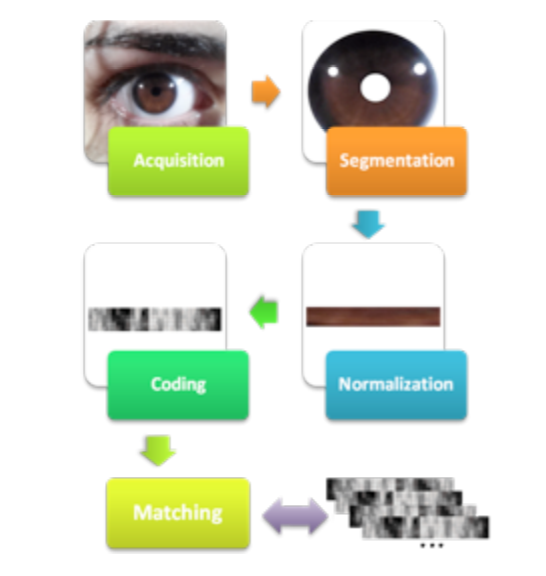
\includegraphics[width=90mm]{img/1/bio_1_1.PNG}
	\caption{\fontsize{10px}{0mm}\selectfont Sequenza delle fasi utili al riconoscimento dell'iride \label{fig:bio_1_1}}
\end{figure}
\section{Obiettivi}
\vspace{8mm}
Gli obiettivi sono quindi la realizzazione di metodologie per effettuare acquisizione, segmentazione, normalizzazione e coding dell'iride in contesti non controllati, in particolare, esse saranno implementate utilizzando un dispositivo comune quale la webcam.
Le metodologie in questione faranno parte di un sistema in grado di utilizzare le metodologie precedenti e capace quindi di ottenere, in particolare, riconoscimento, segmentazione e coding dell'iride.\newpage
		\selectlanguage{italian}
\graphicspath{ {img/2/} }
\chapter{Artificial Intelligence e Machine Learning}\label{cap:CenniAIeML}
\thispagestyle{empty} %Elimina il numero della prima pagina del capitolo.
\newpage

\section{L'\acf{AI}}
\vspace{8mm}
Nella sua accezione più semplice, l'intelligenza artificiale (AI) si riferisce a sistemi o macchine che imitano l'intelligenza umana per eseguire determinate attività e che sono in grado di migliorare continuamente in base alle informazioni raccolte. L'intelligenza artificiale si manifesta in varie forme. Di seguito sono riportati alcuni esempi:

\begin{itemize}
    \item I \textbf{chatbot} utilizzano l'intelligenza artificiale per comprendere più rapidamente i problemi dei clienti e fornire risposte più efficaci. 
    \item Gli \textbf{assistenti intelligenti} utilizzano l'intelligenza artificiale per analizzare le informazioni importanti provenienti da una grande quantità di dati testuali per migliorare la pianificazione.
    \item I \textbf{motori di raccomandazione} possono fornire consigli automatici per programmi TV in base alle abitudini televisive degli utenti.
\end{itemize}

L'intelligenza artificiale fornisce i processi e le capacità per potenziare al massimo la riflessione e l'analisi dei dati. Lo scopo dell'intelligenza artificiale è quello di migliorare in modo significativo le abilità e le attività degli esseri umani. Per questo motivo, è una risorsa molto preziosa per le aziende.

Il termine "intelligenza artificiale" viene utilizzato in modo generico per indicare le applicazioni che eseguono attività complesse che in passato richiedevano l'intervento umano, come comunicare con i clienti online o giocare a scacchi. Il termine viene spesso utilizzato in maniera interscambiabile con i termini \emph{Machine Learning} e \emph{Deep Learning}. Tuttavia, ci sono delle differenze: ad esempio, il Machine Learning è incentrato sulla creazione di sistemi che apprendono o migliorano le loro performance in base ai dati che utilizzano. È importante notare che, sebbene il Machine Learning sia sempre definibile come intelligenza artificiale, l'intelligenza artificiale non è sempre equivalente al Machine Learning.

Per sfruttare appieno il valore dell'intelligenza artificiale, molte aziende stanno investendo in modo significativo in team addetti al data science. \emph{Data science} è un settore interdisciplinare che utilizza metodi scientifici per estrarre valore dai dati e combina le competenze di settori quali la statistica e l'informatica con le conoscenze aziendali per analizzare i dati raccolti da più fonti.

Il fondamento su cui poggia l'intelligenza artificiale, ovvero la capacità di replicare e superare il modo in cui gli umani percepiscono e reagiscono al mondo, sta diventando rapidamente la pietra miliare dell'innovazione. Grazie al Machine Learning, che riconosce gli schemi nei dati e permette di fare previsioni, l'intelligenza artificiale potrà raggiungere notevoli traguardi.

La tecnologia AI sta migliorando le performance e la produttività delle aziende grazie all'automazione dei processi o delle attività che in passato richiedevano l'intervento umano. Inoltre, l'intelligenza artificiale può sfruttare i dati a un livello che nessun essere umano potrebbe mai raggiungere.
\cite{introAI}

\newpage
\section{Machine Learning}
\vspace{8mm}

Il Machine Learning è un sottoinsieme dell'intelligenza artificiale (AI) che si occupa di creare sistemi che apprendono o migliorano le performance in base ai dati che utilizzano. Intelligenza artificiale è un termine generico e si riferisce a sistemi o macchine che imitano l'intelligenza umana. I termini Machine Learning e Intelligenza Artificiale vengono spesso utilizzati insieme e in modo interscambiabile, ma non hanno lo stesso significato. Un'importante distinzione è che sebbene tutto ciò che riguarda il Machine Learning rientra nell'intelligenza artificiale, l'intelligenza artificiale non include solo il Machine Learning.

Attualmente, il Machine Learning è utilizzato in qualsiasi contesto. Quando interagiamo con le banche, acquistiamo online o utilizziamo i social media, vengono utilizzati algoritmi di Machine Learning per rendere la nostra esperienza efficiente, facile e sicura. Il Machine Learning e le tecnologie ad esso associate si stanno sviluppando rapidamente e le loro funzionalità sono in continua evoluzione.

Gli algoritmi sono i motori che alimentano il Machine Learning. I due tipi principali di algoritmi di ML attualmente utilizzati sono gli \emph{algoritmi supervisionati} e gli \emph{algoritmi non supervisionati}. La differenza tra questi due tipi viene definita dal modo in cui ciascun algoritmo apprende i dati per fare previsioni.

\newpage\textbf{Machine Learning supervisionato}\newline	
Gli algoritmi di Machine Learning supervisionato sono i più utilizzati. Con questo modello, un Data Scientist agisce da guida e insegna all'algoritmo i risultati da generare. Esattamente come un bambino impara a identificare i frutti memorizzandoli in un libro illustrato, nel Machine Learning supervisionato l'algoritmo apprende da un set di dati già etichettato e con un output predefinito.

Esempi di algoritmi di Machine Learning supervisionato sono gli algoritmi di regressione lineare e logistica, di classificazione multiclasse e le macchine a vettori di supporto.\newline

\textbf{Machine Learning non supervisionato}\newline
Il Machine Learning non supervisionato utilizza un approccio più indipendente, in cui un computer impara a identificare processi e schemi complessi senza la guida attenta e costante di una persona. Il Machine Learning non supervisionato implica una formazione basata su dati privi di etichette e per i quali non è stato definito un output specifico.

Utilizzando ancora una volta la precedente analogia, il Machine Learning non supervisionato è simile a un bambino che impara a identificare i frutti osservando i colori e gli schemi, anziché memorizzando i nomi con l'aiuto di un insegnante. Il bambino cercherà le somiglianze tra le immagini e le suddividerà in gruppi, assegnando a ciascun gruppo la nuova etichetta corrispondente.

Esempi di algoritmi di Machine Learning non supervisionato
sono gli algoritmi di clustering k-means, l'analisi di componenti principali e indipendenti e le regole di associazione.

Un'altra straordinaria caratteristica del Machine Learning è la sua capacità predittiva. In passato, le decisioni aziendali venivano spesso prese sulla base di risultati storici. Oggi, il Machine Learning utilizza analisi dei dati avanzate per eseguire previsioni. Le organizzazioni possono prendere decisioni proattive e lungimiranti anziché fare affidamento sui dati passati.

Ad esempio, la manutenzione predittiva può consentire ai produttori, alle aziende energetiche e ad altri settori di prendere l'iniziativa e verificare che le loro operazioni rimangano affidabili e ottimizzate. In un giacimento petrolifero con centinaia di trivelle in funzione, i modelli di Machine Learning possono individuare apparecchiature a rischio di malfunzionamento a breve termine e quindi avvisare i team di manutenzione in anticipo. Questo approccio non solo ottimizza la produttività, ma aumenta le performance delle risorse, dei tempi di attività e la durata delle apparecchiature. Può inoltre ridurre al minimo i rischi per i lavoratori.
\cite{introML}

\newpage
\section{Data, Datasets e Preprocessing}
\vspace{8mm}
\subsection{Data}
I metodi di \acf{ML} apprendono dagli esempi. È importante avere una buona conoscenza dei dati di input e delle varie terminologie utilizzate nella descrizione dei dati. Di seguito è riportata la terminologia fondamentale e necessaria per comprendere al meglio i dati utilizzati per algoritmi di Machine Learning.

\begin{itemize}
    \item \textbf{Istanza}: Una singola riga di dati è chiamata istanza. È un'osservazione dal dominio
    \item \textbf{Feature}: Una singola colonna di dati è chiamata feature. È una componente di un'osservazione ed è anche chiamata attributo di un'istanza di dati. Alcune feature possono essere input per un modello, altre possono essere output o feature da prevedere.
    \item \textbf{Data Type}: Le feature hanno un tipo di dati. Possono essere reali o interi o avere un valore categorico o ordinale. Possono essere stringhe, date, orari e tipi più complessi, ma in genere vengono ridotti a valori reali o categorici quando si lavora con i metodi di Machine Learning tradizionali.
    \item \textbf{Dataset}: Una raccolta di istanze è un set di dati. Quando si lavora con metodi di Machine Learning sono necessari alcuni set di dati per scopi diversi.
\end{itemize} 

In genere, per ottenere un modello di Machine Learning, in particolare nel caso del software prodotto, ossia un modello  di classificazione binaria a partire da immagini, viene utilizzato un Dataset contenente sia immagini specifiche, riguardanti il tipo di oggetto da classificare, che immagini non specifiche in cui non è presente l'oggetto da classificare. Questi dati sono quindi accompagnati da etichette o \emph{label} il cui scopo è quello di indicare \emph{l'output corretto} al modello, durante la fase di training.
\begin{figure}[h!]
	\centering
	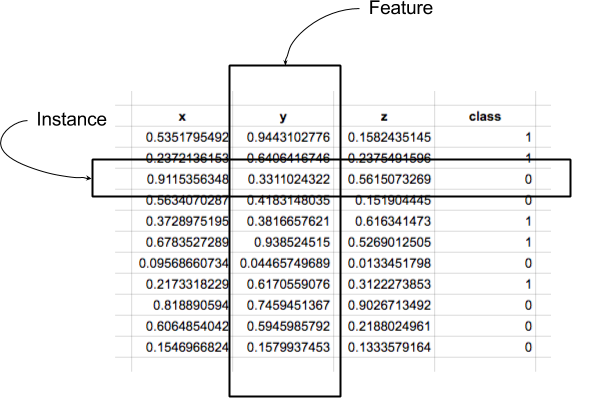
\includegraphics[width=120mm]{img/2/ds_1_1.png}
	\caption{\fontsize{10px}{0mm}\selectfont Istanze e Feature\label{fig:ds_1_1}}
\end{figure}\newline
\subsection{Dataset}
I Dataset, come descritto precedentemente, sono una raccolta di istanze (righe di dati). I Dataset possono essere strutturati o non strutturati. Si parla di \emph{Dataset strutturato} quando i dati in esso contenuti sono conservati in database, organizzati secondo schemi e tabelle rigide. Si parla di \emph{Dataset non strutturato} quando i dati sono conservati senza alcuno schema particolare. Nel caso dei Dataset non strutturati, i sistemi di gestione di dati utilizzabili sono quelli basati sul modello dell’information retrieval.
Alcuni esempi di Dataset strutturati sono i Dataset organizzati secondo strutture quali \ac{CSV}, \ac{TSV}, \ac{JSON}, \ac{XML}, \ac{HTML} e \ac{SQL}.
Nel caso del software sviluppato, i dati sono \textit{non strutturati} poichè si ha a che fare con immagini non conservate in alcun tipo di struttura e senza una particolare organizzazione.

\subsection{Preprocessing}
Quando si affronta un problema di Machine Learning il primo passo consiste nel predisporre di un buon Training set(dataset utilizzato unicamente per la fase di training) a partire dai dataset disponibili in maniera tale da costruire un modello accurato.

É quindi necessaria un’analisi preliminare il cui scopo è quello di evidenziare eventuali criticità e ristrutturare i dati in modo da eliminarne criticità individuate.

Un esempio pratico riguarda la verifica della presenza di valori nulli rispetto alle feature. Dal momento che questi possono compromettere la qualità del modello occorre eliminarli. É possibile procedere in due modi:

\begin{enumerate}
    \item Rimuovere gli esempi con valori 
    \item Sostituire i valori nulli con altri calcolati in maniera opportuna (media della relativa colonna)
\end{enumerate}
Nei problemi di classificazione si ha spesso a che fare con categorie non numeriche che possono creare problemi. Occorre mappare opportunamente le classi con valori ordinali.

Nel caso di valori numerici è abbastanza comune ricorrere alla normalizzazione e alla standardizzazione dei dati.
\newpage
La normalizzazione consente di mappare i valori nell’intervallo [0,1] e si ottiene trasformando ciascun datapoint $x_i$ in

$$x_i = \frac{x_i-x_{min}}{x_{max} - x_{min}}$$

dove $x_{min}$ e $x_{max}$ sono rispettivamente il minimo e il massimo dell’intervallo di partenza.

La standardizzazione punta a centrare i dati intorno allo 0 e a scalarli tenendo presente la deviazione standard.

Ciascun $x_i$ diventa

$$x_i = \frac{x_i-\mu}{\sigma}$$

dove $\mu$ è la media e $\sigma$ è la deviazione standard.

Naturalmente queste trasformazioni agiscono solo sull’intervallo dei dati ma non sulla loro distribuzione che resta inalterata.\cite{preprocessing}\newpage

\section{Problematiche legate alla fase di Training}

Quando si parla di Training si intende "adattamento" ai dati o "apprendimento" dai dati. Durante questa fase il modello inizia ad apprendere a partire dai dati forniti. Questo passaggio è fondamentale poiché l'output finale (o previsione) del modello si baserà sulla capacità del modello di acquisire i pattern dei dati di addestramento.

Un training improprio può portare a un drastico degrado delle prestazioni del modello al momento dell'implementazione. Visti ad alto livello, esistono due tipi principali di risultati della formazione impropria: \emph{underfitting} e \emph{overfitting}.

\subsection{Underfitting}
Quando la complessità del modello è troppo ridotta perché esso apprenda i dati forniti come input, il modello si dice sia in "Underfit". In altre parole, un modello eccessivamente semplice non riesce ad apprendere le tendenze sottostanti ai dati in input. Tale risultato è causato da un modello con bassa varianza\footnote{La varianza di una variabile statistica è una funzione che fornisce una misura della variabilità dei valori assunti dalla variabile stessa} e bias elevato.\newline
Visualizzare graficamente un modello in underfitting può essere di aiuto nel determinare se il modello non fornisce dati adeguati durante il training.
Il seguente grafico mostra un modello il cui scopo è quello di \emph{classificare} i dati nelle classi \textit{Croce} e \textit{Cerchio}

\begin{figure}[h!]
	\centering
	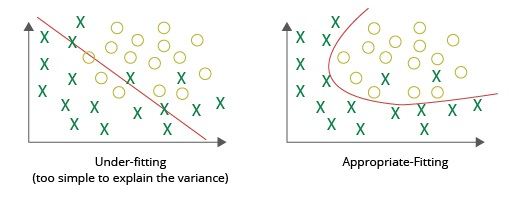
\includegraphics[width=120mm]{img/2/underover_1_1}
	\caption{\fontsize{10px}{0mm}\selectfont Underfitting in un task di classificazione\label{fig:underover_1_1}}
\end{figure}
\newpage
\subsection{Overfitting}
Quando la complessità del modello è troppo elevata rispetto ai dati che sta cercando di apprendere, il modello si dice sia in "Overfit". In altre parole, aumentando la complessità del modello, esso tende ad adattarsi ai noisy data\footnote{Dati con un'abbondanza di informazioni addizionali. Dati corrotti o disturbati.} presente e agli outliers\footnote{Dati che deviano in maniera significativa rispetto al resto dei dati, possono essere causati da errori di misurazione.} presenti nei dati. Il modello ha appreso troppo e quindi non è più in grado di generalizzare.
Tale risultato è causato da un modello con alta varianza e basso bias.\cite{underfitoverfit}\newline
Di seguito è mostrato un modello in overfit utilizzando il precedente esempio.

\begin{figure}[h!]
	\centering
	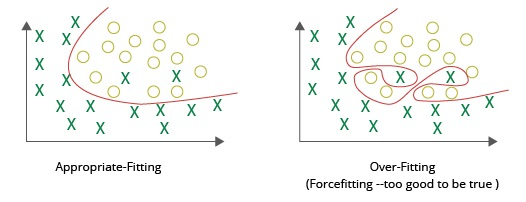
\includegraphics[width=120mm]{img/2/underover_1_2}
	\caption{\fontsize{10px}{0mm}\selectfont Overfitting in un task di classificazione\label{fig:underover_1_2}}
\end{figure}
\newpage

		\selectlanguage{italian}
\graphicspath{ {img/3/} }
\chapter{Neural Network e Convolutional Neural Network}\label{cap:NNeCNN}
\thispagestyle{empty} %Elimina il numero della prima pagina del capitolo.
\newpage

\section{\acf{NN}}
\vspace{8mm}


Ispirate dalla struttura del cervello, le \acf{NN} sono la risposta per rendere i computer capaci di compiere attività tipicamente svolte dall'uomo.
\subsection{Cosa sono le Neural Network?}

I cervelli umani interpretano il contesto delle situazioni del mondo reale in una maniera non concepibile dalle macchine. Le reti neurali furono sviluppate per la prima volta negli anni '50 per affrontare questo problema. Una rete neurale artificiale è un tentativo di simulare la rete di neuroni che formano un cervello umano in modo che il computer sia in grado di apprendere e prendere decisioni in modo umano. Le reti neurali vengono create programmando computer in maniera tale da comportarsi come se fossero cellule cerebrali interconnesse.
\subsection{Come funzionano le Neural Network?}

Le reti neurali artificiali utilizzano diversi livelli di elaborazione matematica per dare un senso alle informazioni che vengono fornite. Tipicamente, una rete neurale artificiale dispone di un numero variabile di neuroni artificiali, da dozzine a milioni di essi. I neuroni artificiali vengono chiamati unità, e sono disposti in una serie di strati. Il livello di input riceve varie forme di informazioni dal mondo esterno, tali informazioni sono i dati che la rete intende elaborare o conoscere. Dall'unità di input, i dati passano attraverso una o più unità nascoste. Il compito dell'unità nascosta è trasformare l'input in qualcosa che l'unità di output può usare.

La maggior parte delle reti neurali è completamente connessa da uno strato all'altro. Queste connessioni sono ponderate: maggiore è il numero, maggiore è l'influenza che un'unità ha su un'altra, simile a un cervello umano. Man mano che i dati passano attraverso ciascuna unità, la rete impara di più sui dati. Dall'altro lato della rete si trovano le unità di output: è qui che la rete risponde ai dati che sono stati forniti e processati.

Affinché le reti neurali possano apprendere, devono disporre di un'enorme quantità di informazioni che fanno parte del training set. Ad esempio, quando si cerca di insegnare ad una rete neurale come differenziare un gatto da un cane, il training set conterrà migliaia di immagini etichettate come immagini di cani e migliaia di immagini etichettate come immagini di gatti in modo da poter insegnare alla rete neurale tale differenza.


Una volta finita la fase di training, il modello prodotto proverà a classificare i dati futuri in base a ciò che viene percepito nelle diverse unità. Durante il periodo di addestramento, l'output della macchina viene confrontato con la descrizione fornita dall'uomo di ciò che dovrebbe essere osservato. Se sono uguali, la macchina è convalidata. Se non corrispondono, vengono utilizzate tecniche per regolare il suo apprendimento, andando indietro attraverso i livelli per modificare l'equazione matematica.
\newline
\begin{figure}[h!]
	\centering
	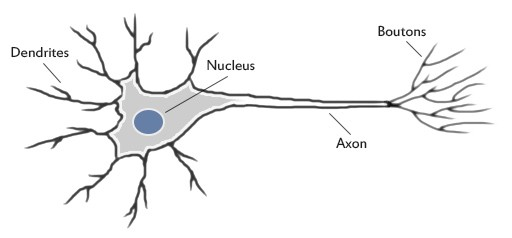
\includegraphics[width=100mm]{img/3/nn_1_1}
	\caption{\fontsize{10px}{0mm}\selectfont Biological Neuron \label{fig:nn_1_2}}
\end{figure}

\newpage
\subsection{Come modelliamo i neuroni artificiali?}

\begin{figure}[h!]
	\centering
	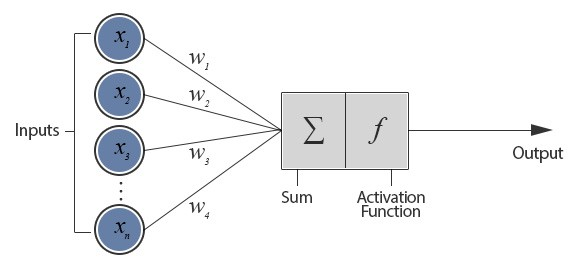
\includegraphics[width=100mm]{img/3/nn_1_2}
	\caption{\fontsize{10px}{0mm}\selectfont Artificial Neuron \label{fig:nn_1_2}}
\end{figure}



La figura rappresenta un neurone artificiale collegato con n altri neuroni artificiali che quindi riceve n input ($x_1$, $x_2$, ... $x_n$). Questa configurazione è chiamata \textbf{Perceptron}.
Gli ingressi ($x_1$, $x_2$,…. $x_n$) e i pesi ($w_1$, $w_2$,…. $w_n$) sono numeri reali che possono essere positivi o negativi.
Il Perceptron è costituito da pesi, da un processore di somma, da una funzione di attivazione e da un processore di soglia (noto come \textbf{bias}).
Il \textit{bias} di un algoritmo è l'insieme di assunzioni che il modello utilizza per prevedere gli output in base agli input non familiari, ossia non ancora incontrati, i pesi (\textit{weights}) invece sono delle costanti che indicano l'importanza della variabile associata nel determinare il valore dell'output del modello.

Tutti gli ingressi sono pesati individualmente, sommati e passati alla funzione di attivazione. Esistono molti tipi distinti di funzioni di attivazione, ma una delle più semplici è la funzione a gradini. Una funzione a gradini genererà output 1 se l'ingresso è superiore a una determinata soglia, altrimenti genererà output 0.
\newpage
Successivamente, verranno presentati i \textit{vettori di input} ottenuti da un training set, il Perceptron modificherà i pesi in base alla seguente equazione:


$$ \forall i \; W(i) = W(i) + A(T-A)*P(i) $$ 

Nota: in realtà l'equazione è 
$$W(i) = W(i) + a*g’*(T-A)*P(i)$$
dove $g’$ è la derivata della funzione di attivazione ed $a$ è il learning rate.
Il calcolo della derivata di una funzione a gradini può diventare complicato, inoltre esso non è di fondamentale importanza nella comprensione del topic in questione, quindi tale calcolo verrà ignorato.

$W$ è il vettore dei pesi, $P$ è il vettore di input, $T$ è l'output corretto che il Perceptron avrebbe dovuto conoscere e $A$ è l'ouput dato dal Perceptron stesso.

Quando tutti i vettori di training sono stati presentati al Perceptron e non si presentano errori, allora esso è stato allenato con successo.\newpage

\subsection{Cosa avviene nel Perceptron?}
Il perceptron, di volta in volta, somma tutti gli input e li separa in 2 categorie, quelli che causano un \emph{segnale di fire}\footnote{il nome deriva dalla biologia: quando i neuroni inviano un segnale nel cervello, si parla di firing} e quelli che non lo causano. Cioè, sta "disegnando" la linea:
$$w_1x_1 + w_2x_2 = t$$
I punti su un lato della linea rientrano in una categoria, i punti sull'altro lato rientrano nell'altra categoria.
La linea ottenuta è solo una delle infinite linee che possono essere ottenute per la separazione delle categorie.
\newline
\textbf{Limiti dei Perceptron}\newline
Non tutti gli insiemi di input possono essere divisi attraverso una linea. Nel caso in cui sia possibile, si parla di input \textit{linearmente separabili}. Se i vettori non sono linearmente separabili, la fase di apprendimento non raggiungerà mai un punto in cui tutti i vettori sono classificati in maniera corretta, e bisognerà utilizzare un approccio diverso.
\cite{MediumNN}
\newpage

\section{\acf{CNN}}
\vspace{8mm}
Le \acf{CNN} sono una categoria di reti neurali che si sono dimostrate molto efficaci in settori quali il riconoscimento e la classificazione delle immagini.
Le CNN, come le reti neurali (NN), sono costituite da neuroni con pesi e bias. Ogni neurone riceve diversi input, ne prende una somma, la passa attraverso una funzione di attivazione e risponde con un output, in pratica sembrano essere equivalenti alle reti neurali.
Diviene quindi naturale porsi la domanda: \textbf{Qual è la differenza tra CNN e NN?}\newline
Tra le varie differenze, la risposta è data dal fatto che le CNN hanno una caratteristica fondamentale: \textit{lavorano su volumi}, ossia, invece di ricevere in input un vettore di valori, ricevono in input un immagine, che è composta quindi da 3 vettori, uno per dimensione.

\newpage
\subsection{Convolution e funzionamento}

Per capire al meglio il funzionamento delle \acf{CNN} bisogna comprendere il concetto di \textbf{Convolution}(da cui il nome). Per farlo, utilizzeremo un filtro di dimensione arbitraria, in questo caso le dimensioni saranno 5x5x3.\newline
\begin{figure}[h!]
	\centering
	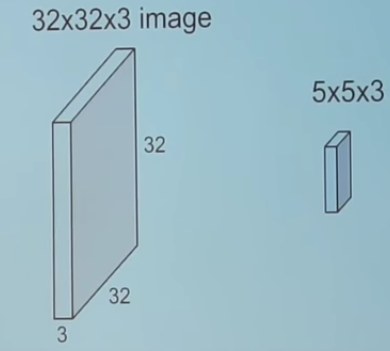
\includegraphics[width=80mm]{img/3/cnn_1_1}
	\caption{\fontsize{10px}{0mm}\selectfont Immagine e filtro considerati \label{fig:cnn_1_1}}
\end{figure}
\newpage
Una volta ottenuto il filtro, lo si fa scorrere sopra l'intera immagine e di volta in volta si calcola il prodotto tra il filtro e le sezioni dell'immagine sulle quali ci si trova, il risultato del prodotto sarà uno scalare.
\begin{figure}[h!]
	\centering
	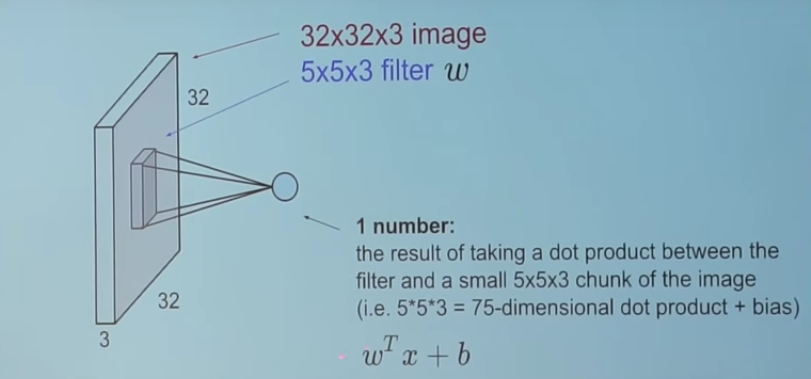
\includegraphics[width=110mm]{img/3/cnn_1_2}
	\caption{\fontsize{10px}{0mm}\selectfont Il prodotto appena descritto \label{fig:cnn_1_2}}
\end{figure}
\newline
Una volta calcolati tutti i prodotti si otterrà il seguente risultato:
\begin{figure}[h!]
	\centering
	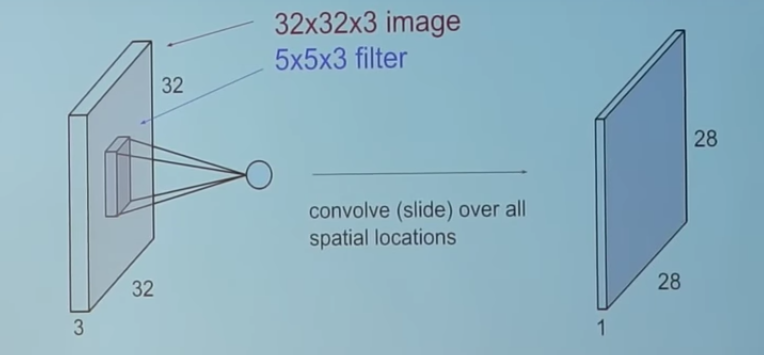
\includegraphics[width=110mm]{img/3/cnn_1_3}
	\caption{\fontsize{10px}{0mm}\selectfont Risultato finale \label{fig:cnn_1_3}}
\end{figure}
\newpage
Tornando alle CNN, si utilizza un cosiddetto \textbf{Convolutional Layer}(strato convoluzionale) che costituisce la parte fondamentale di una Convolutional Neural Network.
\begin{figure}[h!]
	\centering
	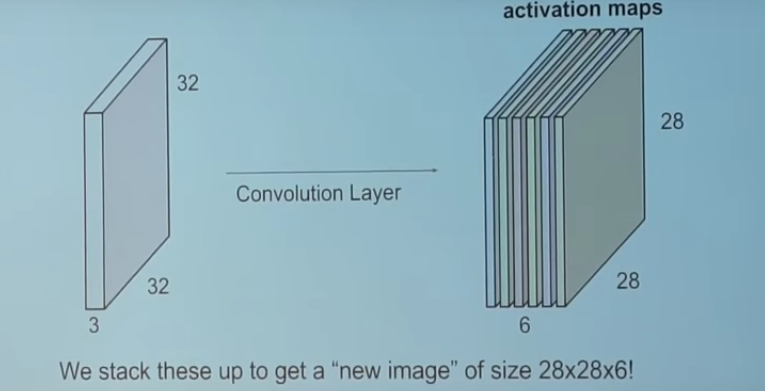
\includegraphics[width=110mm]{img/3/cnn_1_4}
	\caption{\fontsize{10px}{0mm}\selectfont Convolutional Layer \label{fig:cnn_1_4}}
\end{figure}
\newline
Lo strato convoluzionale contiene un insieme di filtri indipendenti(6 nell'esempio mostrato). Ogni filtro è convoluto con l'immagine indipendentemente dagli altri, risultando quindi in 6 \textit{feature maps} differenti(una feature map non è altro che l'output dell'applicazione del layer all'immagine).\cite{MediumCNN}

\subsection{Perchè non è stato utilizzato CNN?}\label{considerazioniCNN}
Come già detto precedentemente, le reti neurali convoluzionali sono una categoria di reti neurali molto efficaci per task di classificazione delle immagini. Nonostante ciò, durante l'attività di progettazione del software, in particolare durante la ricerca di Dataset contenenti immagini di iridi per il training della CNN, è stata riscontrata una notevole mancanza di dati: il dataset finale contiene 2500 immagini, da dividere in training set e test set, un numero piuttosto basso.
Tutto ciò, insieme alla estrema specificità dei dati causa overfitting da parte della CNN utilizzata, è stato quindi utilizzato un nuovo approccio: \emph{Viola-Jones} e \emph{Haar Cascades}
\newpage
		\selectlanguage{italian}
\graphicspath{ {img/4/} }
\chapter{Viola Jones e Haar Cascades}\label{cap:ViolaHaar}
\thispagestyle{empty} %Elimina il numero della prima pagina del capitolo.
\newpage

\section{Viola Jones}
\vspace{8mm}

La classificazione delle immagini è un campo in rapida crescita e l'utilizzo delle reti neurali convoluzionali (CNN) e di altre tecniche di apprendimento è in rapida crescita.
Tuttavia, prima che le CNN diventassero di utilizzo comune, un'altra tecnica era ampiamente utilizzata e continua ad essere utilizzata: \emph{Viola-Jones}.
Mentre una CNN è un singolo classificatore che osserva un'immagine per intero e applica operazioni matriciali per arrivare a una classificazione, Viola-Jones adotta un approccio d'insieme. Ciò significa che Viola-Jones utilizza molti classificatori diversi, ognuno dei quali osserva una diversa porzione dell'immagine. Ogni singolo classificatore è più debole (meno accurato, produce più falsi positivi) rispetto al classificatore finale perché riceve meno informazioni. Quando i risultati di ciascun classificatore vengono combinati, tuttavia, viene prodotto un classificatore forte.

\begin{figure}[h!]
	\centering
	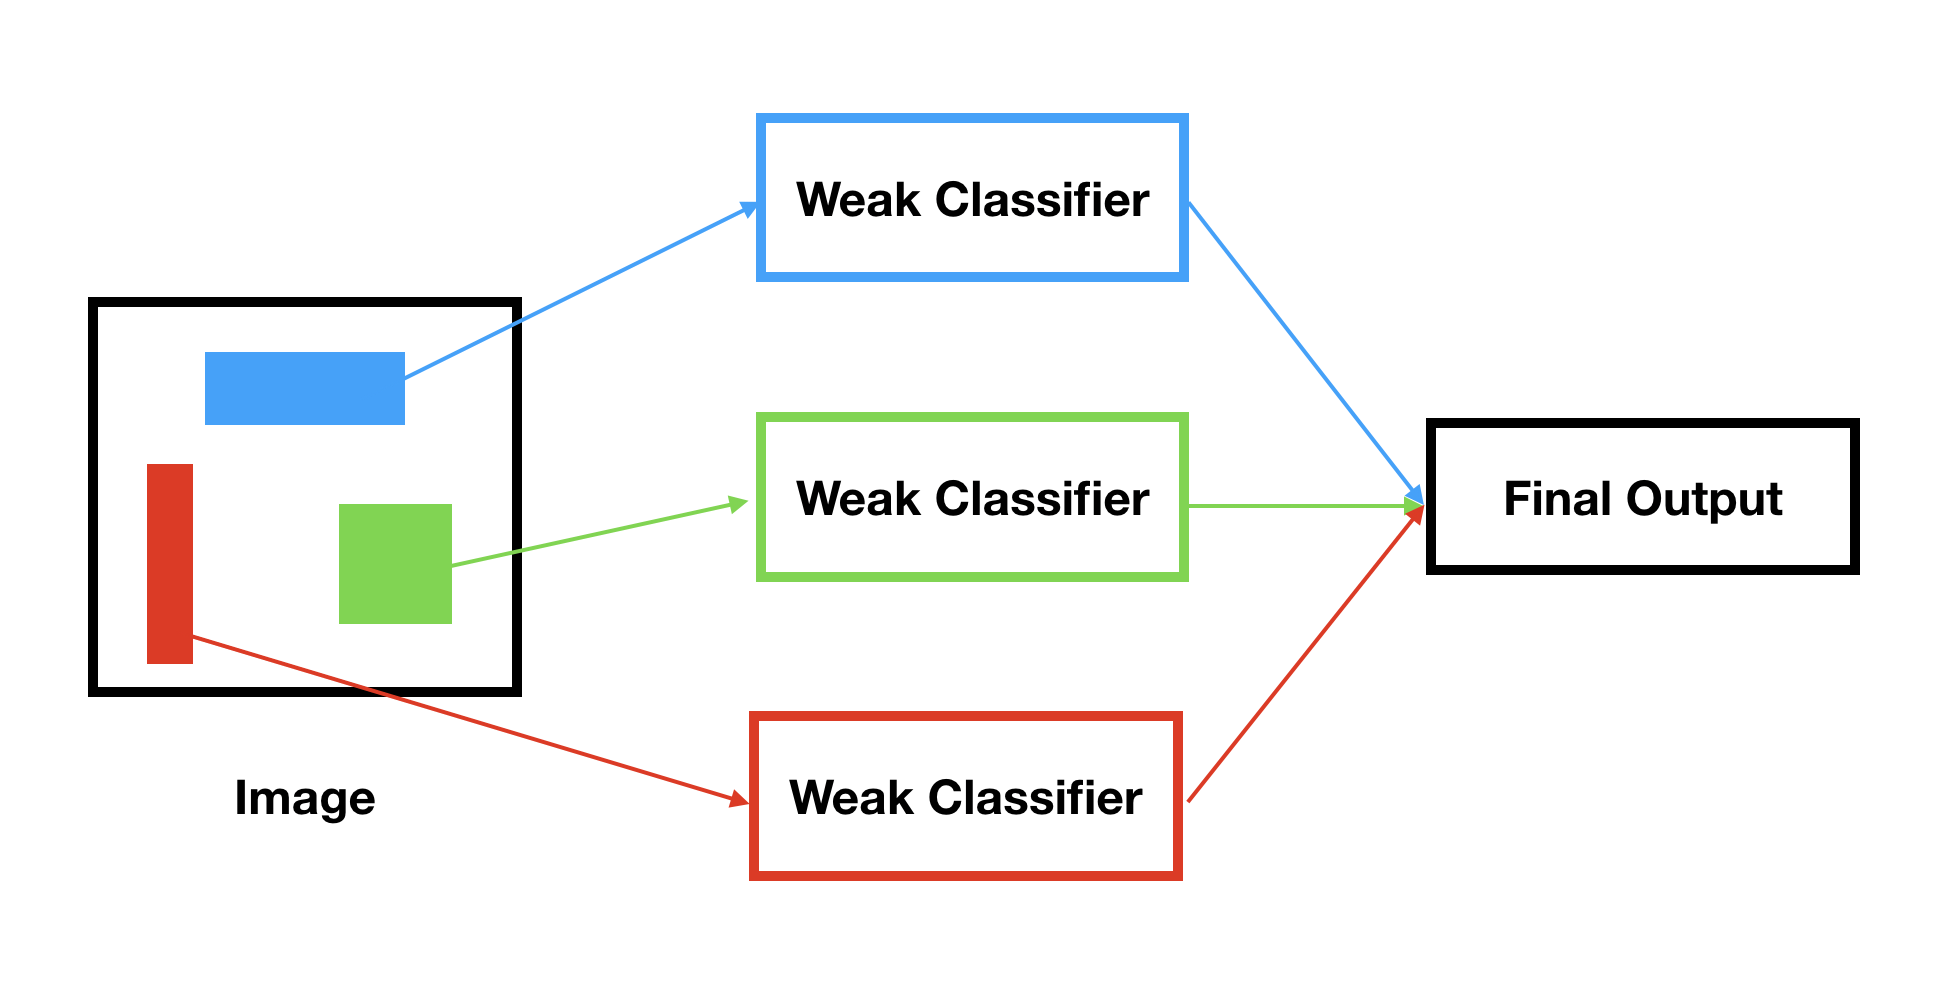
\includegraphics[width=80mm]{img/4/violahaar_1_1}
	\caption{\fontsize{10px}{0mm}\selectfont Classificatori in Viola-Jones \label{fig:violahaar_1_1}}
\end{figure}

A causa della natura dell'algoritmo, il metodo Viola-Jones è limitato alle attività di classificazione binaria (come il rilevamento di oggetti) e ha un periodo di training piuttosto lungo. Tuttavia, esso classifica le immagini rapidamente grazie al fatto che ogni classificatore debole richiede solo un piccolo numero di parametri, inoltre, con un numero sufficiente di classificatori deboli, l'algoritmo ha un basso tasso di falsi positivi\footnote{Un falso positivo è un risultato in cui il modello prevede erroneamente la classe come positiva.}.
\newpage
\subsection{Features e Integral Image}
Uno dei primi contributi chiave apportati nel documento\cite{violapaper} che introduce Viola-Jones è stato un insieme di semplici feature da utilizzare nel riconoscimento delle immagini. Nella maggior parte delle attività, i valori dei pixel sono le caratteristiche immesse nell'algoritmo. Tuttavia, Viola e Jones hanno introdotto le seguenti nuove feature.

\begin{figure}[h!]
	\centering
	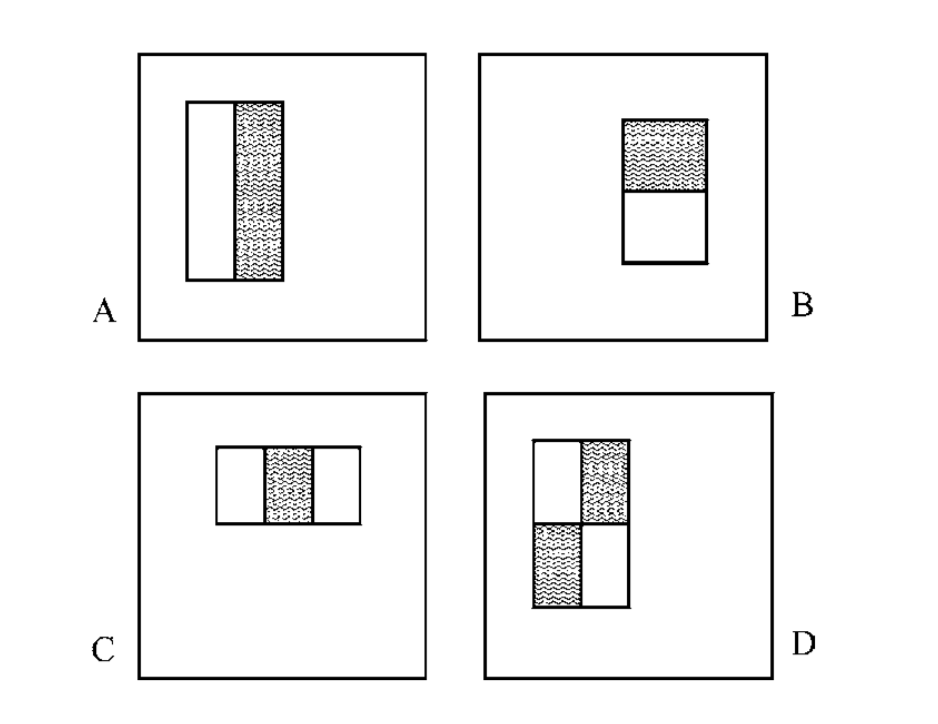
\includegraphics[width=80mm]{img/4/violahaar_1_2}
	\caption{\fontsize{10px}{0mm}\selectfont A e B sono feature a due rettangoli, C è una feature a tre rettangoli e D è una feature a 4 rettangoli. Immagine tratta dal documento originale. \label{fig:violahaar_1_2}}
\end{figure}

La somma dei pixel nei rettangoli non ombreggiati viene sottratta dalla somma dei pixel nei rettangoli ombreggiati. È facile vedere che anche per le immagini di piccole dimensioni ci sono molte feature (oltre 160.000 per un'immagine 24 x 24). Poiché l'algoritmo richiede l'iterazione di tutte le feature, è necessario calcolarle in modo molto efficiente. Per fare questo, Viola e Jones hanno introdotto le \emph{Integral Image}, L'immagine integrale è definita dalla seguente relazione ricorsiva: \newpage

\begin{figure}[h!]
	\centering
	
\includegraphics[width=80mm]{img/4/violahaar_1_3}
	\caption{\fontsize{10px}{0mm}\selectfont Relazione ricorsiva dell'immagine integrale \label{fig:violahaar_1_3}}
\end{figure}
$s(x, y)$ è la somma cumulativa delle righe nel punto $(x, y)$, $ii(x, y)$ è il valore dell'immagine integrale nello stesso punto e $i(x, y)$ è il valore del pixel in quel punto. Questa relazione non dice altro che l'immagine integrale in un punto $(x, y)$ è la somma di tutti i pixel in alto a sinistra rispetto al pixel corrente. Ciò semplifica il calcolo della somma dei pixel in una regione rettangolare come mostrato di seguito.


\begin{figure}[h!]
	\centering
	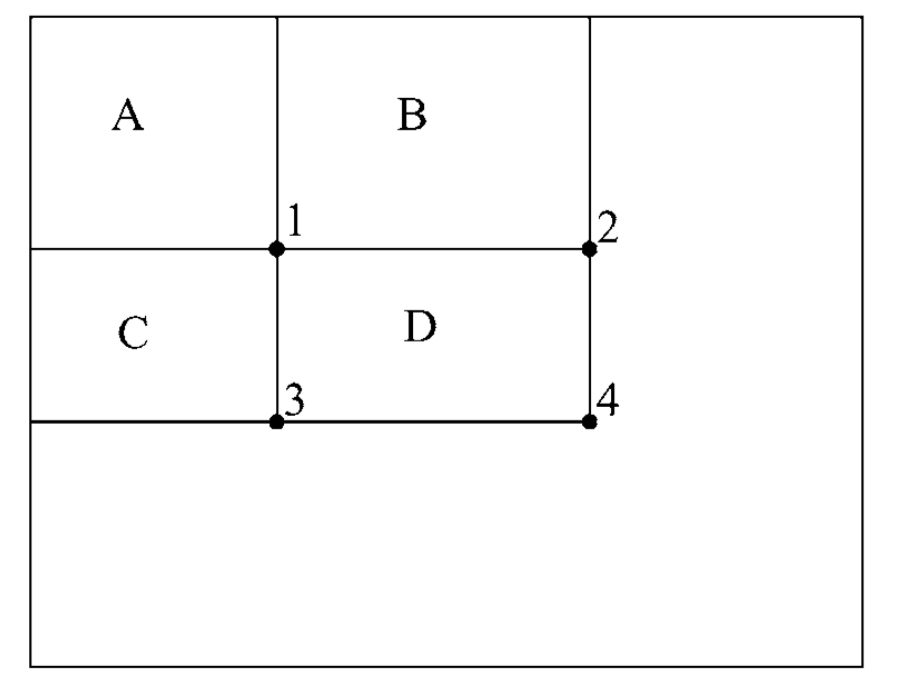
\includegraphics[width=80mm]{img/4/violahaar_1_4}
	\caption{\fontsize{10px}{0mm}\selectfont Calcolo dei pixel in una regione rettangolare \label{fig:violahaar_1_4}}
\end{figure}

La somma dei pixel nella regione $D$ è $ii(4) + ii (1) - ii (2) - ii (3)$ che non sono altro che quattro riferimenti ad array.\newpage

\subsection{Training e Weak Classifiers}

Il ciclo principale di training richiede la scelta del miglior classificatore debole, ma esiste un classificatore debole per ogni possibile caratteristica. Per questo motivo, dobbiamo creare tutte le feature prima di iniziare a implementare il ciclo principale di training.

Quando verranno identificati i classificatori deboli ottimali da utilizzare in seguito nell'algoritmo, sarà necessario valutare ciascuna feature per ogni esempio di training. Per risparmiare computazione, verrà effettuata la valutazione di ogni feature prima di iniziare il training dei classificatori. Questa scelta è più efficiente perché ogni classificatore deve essere riqualificato ogni volta che ne viene selezionato uno nuovo.

Viola-Jones utilizza una serie di classificatori deboli e pondera i loro risultati insieme per produrre la classificazione finale. Ogni classificatore è "debole" perché da solo non può adempiere con precisione all'attività di classificazione. Ogni classificatore debole osserva una singola feature $f$, ha una soglia $\theta$ e una polarità $p$ per determinare la classificazione di un esempio di training.
\begin{figure}[h!]
	\centering
	
\includegraphics[width=80mm]{img/4/violahaar_1_5}
	\caption{\fontsize{10px}{0mm}\selectfont Classificatore debole \label{fig:violahaar_1_5}}
\end{figure}

La polarità può essere -1 o 1. Quando $p=1$, il classificatore debole produce un risultato positivo quando $f(x)<\theta$ o quando il valore della feature è inferiore alla soglia. Quando $p=-1$ il classificatore debole produce un risultato positivo per $f(x)>\theta$.\newpage

Si noti che ogni feature è la somma delle regioni rettangolari positive con la somma delle regioni rettangolari negative sottratte da esse. Il prossimo passo dell'algoritmo è scegliere il miglior classificatore debole. Per fare ciò, dobbiamo trovare la soglia e la polarità ottimali per ognuno di essi.

L'addestramento dei classificatori deboli è la parte più costosa dal punto di vista computazionale dell'algoritmo. Ogni volta che un nuovo classificatore debole viene selezionato come il migliore, tutti gli altri devono essere riqualificati poiché gli esempi di allenamento sono pesati in maniera diversa. Tuttavia, esiste un modo efficiente per trovare la soglia e la polarità ottimali per un singolo classificatore debole utilizzando i pesi. Innanzitutto, si ordinano i pesi in base al valore della feature alla quale corrispondono, dopodiché si scorre attraverso la matrice dei pesi e si calcola l'errore se la soglia è stata scelta per essere quella feature. Infine, si trovano soglia e polarità aventi il minimo errore. I possibili valori per una soglia sono i valori della feature su ciascun esempio di allenamento. L'errore può essere misurato da:

$$ e = \min{(S^+ + T^- - S^-, S^- + T^+ - S^+)} $$

Dove $T$ rappresenta la somma totale dei pesi e $S$ rappresenta la somma dei pesi di tutti gli esempi visti finora. Gli apici $+$ e $-$ indicano a quale classe appartiene la somma. Concettualmente, questo errore confronta quanti esempi verranno classificati in modo errato se tutti gli esempi al di sotto della posizione corrente sono etichettati come negativi con quanti esempi saranno classificati in modo errato se tutti gli esempi al di sotto della posizione corrente sono etichettati come positivi (tenendo conto di come ogni esempio è pesato).

In questa maniera, è possibile valutare l'errore di ogni possibile soglia in tempo costante $(O(1))$ e l'errore di tutte le soglie in tempo lineare $(O(n))$. La soglia è impostata sul valore della feature per cui l'errore è minimo. La polarità è determinata da quanti esempi positivi ed esempi negativi si trovano a sinistra (minore) e a destra(maggiore) della soglia. Se rimangono altri esempi positivi a sinistra della soglia allora $p=1$. Altrimenti, $p=-1$.

\begin{figure}[h!]
	\centering
	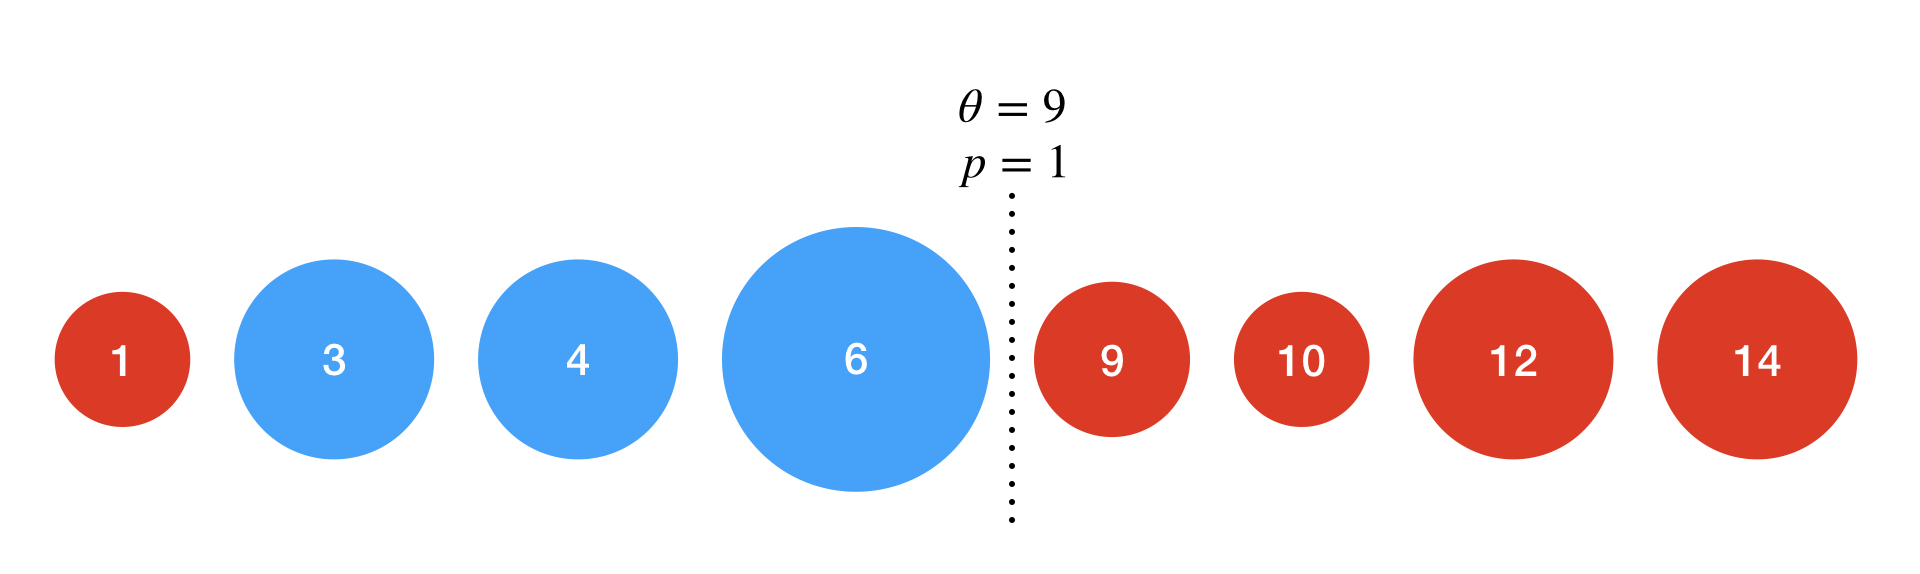
\includegraphics[width=100mm]{img/4/violahaar_1_6}
	\caption{\fontsize{10px}{0mm}\selectfont In questo esempio, i numeri indicano i valori delle feature e la dimensione delle bolle indica i loro pesi relativi. Chiaramente, l'errore verrà minimizzato quando qualsiasi feature con un valore inferiore a 9 viene classificata come blu. Ciò corrisponde a una soglia di 9 con una polarità di 1. \label{fig:violahaar_1_6}}
\end{figure}
Una volta addestrati tutti i classificatori deboli, possiamo trovare il migliore semplicemente scorrendo attraverso tutti i classificatori e calcolando l'errore medio pesato di ciascuno di essi.\newpage

\subsection{Strong Classifier}
L'ultimo passaggio riguarda il classificatore finale. Dobbiamo compilare il classificatore forte a partire dai classificatori deboli. Il classificatore forte è definito come:

\begin{figure}[h!]
	\centering
	
\includegraphics[width=100mm]{img/4/violahaar_1_7}
	\caption{\fontsize{10px}{0mm}\selectfont Definizione classificatore forte \label{fig:violahaar_1_7}}
\end{figure}


Il coefficiente $\alpha$ indica quanto ciascun classificatore debole è rilevante nella decisione finale e dipende dall'errore poiché è il logaritmo naturale dell'inverso di $\beta$. La somma pesata delle decisioni dei classificatori deboli viene confrontata con la metà della somma degli $\alpha$.
\cite{violajones}

\section{Considerazioni riguardanti Viola-Jones}
\vspace{8mm}
In base a quanto descritto finora, la struttura dell'algoritmo di classificazione Viola-Jones rende l'approccio particolarmente robusto sia per la selezione di feature che per la classificazione di immagini. Il documento originale di Viola-Jones introduce vari concetti per ridurre il tempo di classificazione.
Durante la fase di progettazione, quindi, sono state considerate diverse opzioni per ottimizzare l'algoritmo e rendere l'approccio quanto più performante possibile soprattutto in base alle considerazioni descritte nella sezione \ref{considerazioniCNN} riguardanti la mancanza e l'estrema specificità dei dati.
\newpage

\section{Haar Cascades}
\vspace{8mm}

Haar Cascades è un algoritmo di Machine Learning utilizzato per identificare oggetti in un'immagine o in un video. È basato sul concetto di feature proposto da Paul Viola e Michael Jones nel loro articolo "Rapid Object Detection using a Boosted Cascade of Simple Features" nel 2001. L'idea è che viene utilizzata una funzione a cascata, addestrata a partire da immagini positive e negative. Viene utilizzato quindi per rilevare oggetti all'interno di immagini. È noto per essere in grado di rilevare volti e parti del corpo in un'immagine, ma può essere addestrato per identificare quasi qualsiasi oggetto.
\\
L'algoritmo è composto da 4 fasi:

\begin{enumerate}
  \item Haar Feature Selection
  \item Creating Integral Images
  \item Adaboost Training
  \item Cascading Classifiers
\end{enumerate}

\subsection{Haar Feature e Adaboosting}
Prendiamo il rilevamento del volto come esempio. Inizialmente, l'algoritmo necessita di immagini positive di volti e immagini negative senza volti per addestrare il classificatore. Quindi dobbiamo estrarre feature da esso.\newpage

Il primo passo è quello di raccogliere le \emph{Haar Features}. Una Haar Feature considera le regioni rettangolari adiacenti in una posizione specifica in una finestra di rilevamento, somma le intensità dei pixel in ciascuna regione e calcola la differenza tra queste somme. Per rendere questo procedimento molto rapido, vengono utilizzate le \emph{Integral Image}
\begin{figure}[h!]
	\centering
	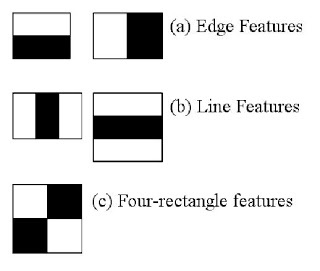
\includegraphics[width=80mm]{img/4/violahaar_1_8}
	\caption{\fontsize{10px}{0mm}\selectfont Haar Feature \label{fig:violahaar_1_8}}
\end{figure}

Si noti che la maggior parte delle feature calcolate è irrilevante. Si consideri l'immagine riportata in seguito. La riga superiore mostra due feature rilevanti. La prima feature selezionata sembra concentrarsi sulla proprietà che la regione degli occhi è spesso più scura della regione del naso e delle guance. La seconda feature selezionata si basa sulla proprietà che gli occhi sono più scuri del ponte del naso. Contemporaneamente, però, le stesse finestre che si applicano sulle guance o in qualsiasi altro posto sono irrilevanti.

\begin{figure}[h!]
	\centering
	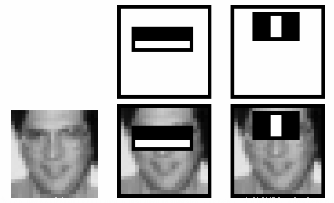
\includegraphics[width=60mm]{img/4/violahaar_1_9}
	\caption{\fontsize{10px}{0mm}\selectfont Esempio di Haar Feature \label{fig:violahaar_1_9}}
\end{figure} \newpage


Come possiamo selezionare le migliori funzionalità tra le oltre 160.000 funzionalità? La risposta a tale domanda risiede in un approccio chiamato \emph{Adaboost}, che seleziona le migliori feature e addestra i classificatori che le usano. Questo algoritmo costruisce un classificatore “forte” come una combinazione lineare di classificatori “deboli” pesati. Il processo è il seguente:

Durante la fase di rilevamento, una finestra della dimensione del target viene spostata sull'immagine di input e per ciascuna sottosezione dell'immagine vengono calcolate le Haar Feature.
Questa differenza viene successivamente confrontata con una soglia appresa che separa gli oggetti della classe di oggetti di interesse da quelli che non vi appartengono. Poiché ogni Haar Feature è solo un "classificatore debole" (la sua qualità di rilevazione è leggermente migliore di una supposizione casuale) è necessario un gran numero di Haar Feature per descrivere un oggetto con sufficiente precisione, di conseguenza si organizzano le Haar Feature in \emph{Cascade Classifiers}(classificatori a cascata) per formare un classificatore forte.

\subsection{Cascade Classifier}

Il classificatore a cascata è costituito da una raccolta di fasi, in cui ogni fase è un insieme di \emph{Weak Learner}. I Weak Learner sono semplici classificatori chiamati \emph{decision stumps}. Per ogni fase il training avviene utilizzando una tecnica nota come \emph{boosting}. Il boosting fornisce la capacità di addestrare un classificatore altamente accurato prendendo una media ponderata delle decisioni prese dai classificatori deboli.

Ogni fase del classificatore identifica la regione definita dalla posizione corrente della finestra scorrevole come positiva o negativa. Positivo indica che è stato trovato un oggetto e negativo indica che non sono stati trovati oggetti. 

Se l'etichetta è negativa, la classificazione di questa regione è completa e il rilevatore fa scorrere la finestra nella \emph{posizione} successiva. Se l'etichetta è positiva, il classificatore passa la regione alla \emph{fase} successiva. Il rilevatore segnala un oggetto trovato nella posizione corrente della finestra quando la fase finale classifica la regione come positiva.

Le fasi sono progettate per rifiutare campioni negativi il più rapidamente possibile. L'ipotesi è che la stragrande maggioranza delle finestre non contenga l'oggetto di interesse. Al contrario, i \emph{true positive} sono rari e vale la pena dedicare del tempo alla verifica.
\begin{itemize}
  \item Un \textbf{true positive} si verifica quando un campione positivo è correttamente classificato.
  \item Un \textbf{false positive} si verifica quando un campione negativo viene erroneamente classificato come positivo.
  \item Un \textbf{false negative} si verifica quando un campione positivo viene erroneamente classificato come negativo.
\end{itemize}

Per un corretto funzionamento, ogni fase della cascata deve avere un basso tasso di false negative. Se una fase etichetta erroneamente un oggetto come negativo, la classificazione si interrompe e non è possibile correggere l'errore. Tuttavia, ogni fase può avere un alto tasso di falsi positivi. Anche se il rilevatore etichetta erroneamente un non-oggetto come positivo, è possibile correggere l'errore nelle fasi successive. L'aggiunta di più fasi riduce il tasso complessivo di false positive, ma riduce anche il tasso complessivo di true positive.

Il training del classificatore a cascata richiede una serie di campioni positivi e una serie di immagini negative. È necessario fornire una serie di immagini positive con le regioni di interesse specificate che verranno utilizzate come campioni positivi. È inoltre necessario fornire un set di immagini negative da cui la funzione genera automaticamente campioni negativi.
\cite{haarcascades}\newpage


\section{Considerazioni riguardanti Haar Cascades}
\vspace{8mm}

In base a quanto descritto nelle precedenti sezioni, un approccio basato sull'algoritmo Haar Cascades può portare ottime prestazioni se utilizzato in maniera corretta.
Rispetto all'approccio basato su Viola-Jones, Haar Cascades si presta più efficiente e più fluido in task di rilevazione di individui \emph{in qualsiasi contesto}.
Nel prossimo capitolo viene mostrato come Haar Cascades è stato utilizzato nella stesura del software.
\newpage
		\selectlanguage{italian}
\graphicspath{ {img/5/} }
\chapter{Realizzazione e sviluppo del software}\label{cap:software}
\thispagestyle{empty} %Elimina il numero della prima pagina del capitolo.
\newpage
\section{L'approccio utilizzato}
\vspace{8mm}
Il software è stato realizzato utilizzando due Haar Cascades attraverso i quali vengono riconosciuti occhi e viso. Gli Haar Cascades utilizzati sono nel formato \ac{XML} e sono distribuiti in maniera \emph{open source} da \emph{Intel Corporation}.
Gli Haar Cascades sono stati utilizzati grazie ai CascadeClassifier forniti all'interno della libreria \emph{OpenCV}.

Il software prodotto, ottenuto attraverso l'impiego del linguaggio di programmazione \emph{Python}, è costituito di due script,  ExtractSector.py e IrisSegmentation.py, che verranno descritti in seguito.
Da un punto di vista ad alto livello, il software ottiene la riproduzione live utilizzando una webcam, tale riproduzione viene analizzata di frame in frame, ogni frame è successivamente portato in grayscale per permettere un'analisi più efficiente.
Una volta fatto ciò, vengono individuati viso, occhi, e iride, e su richiesta dell'utente verrà effettuata la segmentazione, polarizzazione e codifica delle iridi degli occhi.
\begin{figure}[h!]
	\centering
	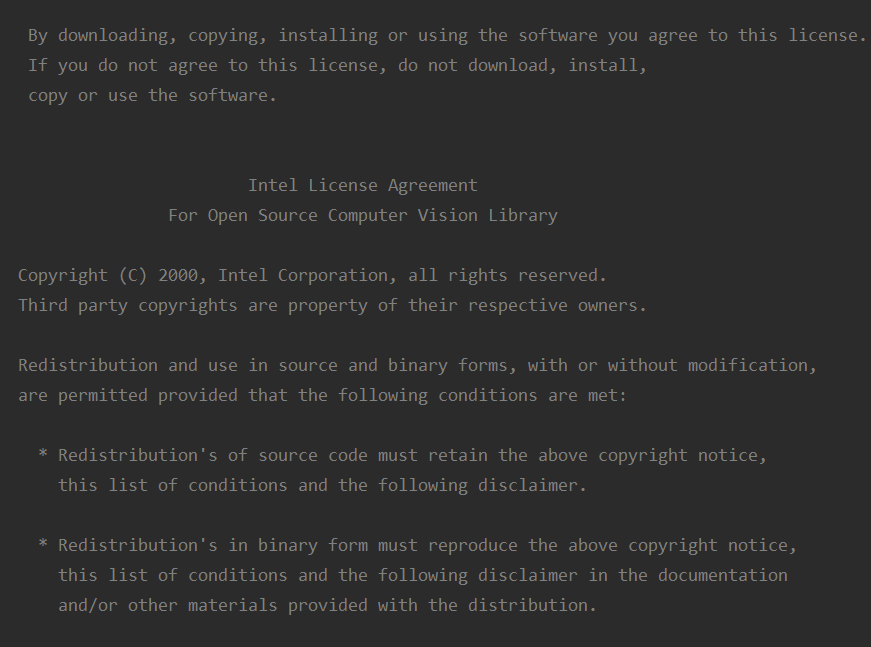
\includegraphics[width=120mm]{img/5/intel1.png}
	\caption{\fontsize{10px}{0mm}\selectfont Intel License Agreement\label{fig:intel_1_1}}
\end{figure} \newpage
\begin{figure}[h!]
	\centering
	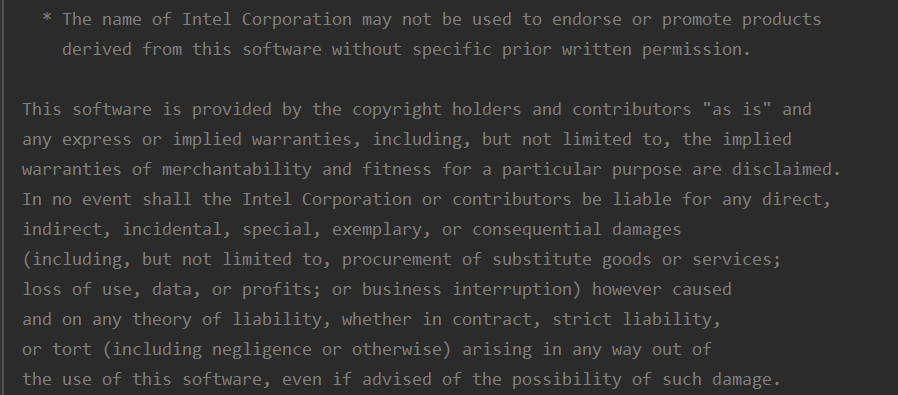
\includegraphics[width=120mm]{img/5/intel2.png}
	\caption{\fontsize{10px}{0mm}\selectfont Intel License Agreement \label{fig:intel_1_2}}
\end{figure}
\newpage
\section{Codice}
\vspace{8mm}
\subsection{Lo script Iris Segmentation}
Iris Segmentation è lo script contenente la maggior parte delle operazioni effettuate dal sistema. Come già accennato precedentemente, vengono utilizzati due Haar Cascades per il riconoscimento di viso e occhi. 
Lo script inizia ottenendo la riproduzione live a partire dalla webcam che verrà mostrata in una finestra, le cui dimensioni sono specificate in riga 12 e 13.

\begin{figure}[h!]
	\centering
	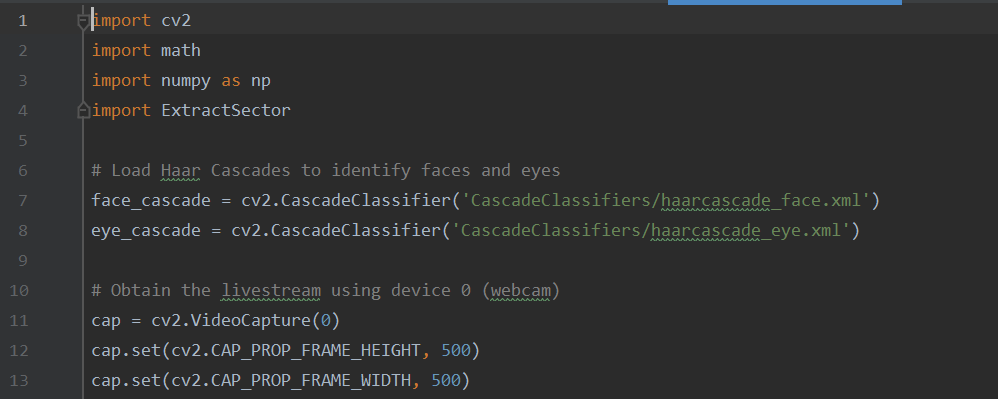
\includegraphics[width=120mm]{img/5/codice_1_1}
	\caption{\fontsize{10px}{0mm}\selectfont Fasi iniziali\label{fig:codice_1_1}}
\end{figure}

Una volta inizializzata la cattura, bisogna prendere le immagini di frame in frame, in un loop infinito, questa operazione viene eseguita attraverso il metodo \emph{read} in riga 17. Come vedremo successivamente, il loop può essere arrestato su input dell'utente.
Ottenute le immagini, introduciamo un concetto chiave, chiamato \emph{roi}, ossia la regione di interesse(region of interest) che viene analizzata in ogni dato istante.
\begin{figure}[h!]
	\centering
	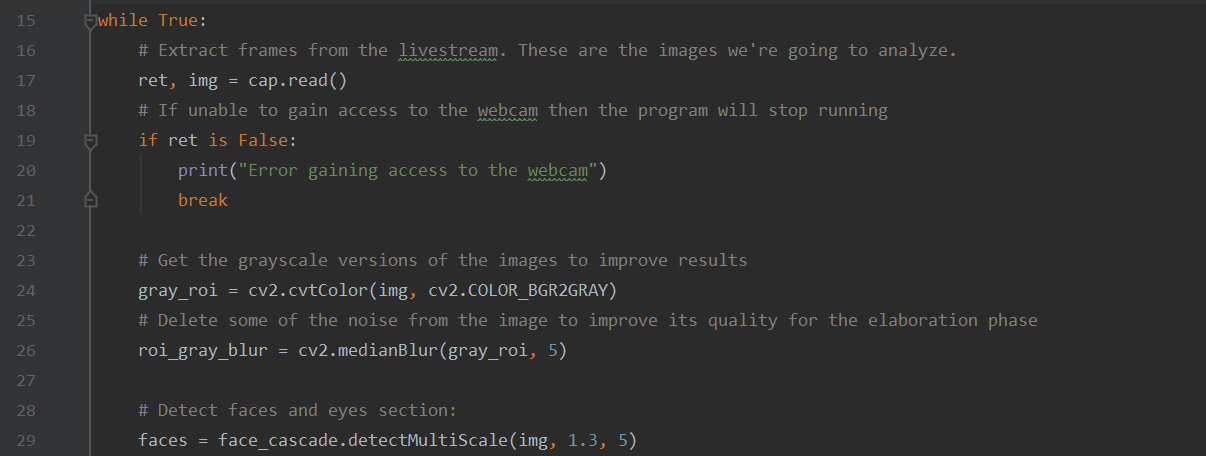
\includegraphics[width=120mm]{img/5/codice_1_2}
	\caption{\fontsize{10px}{0mm}\selectfont Fasi iniziali e processing \label{fig:codice_1_2}}
\end{figure}\newpage

La regione di interesse, inizialmente, corrisponde all'intera immagine, che verrà convertita in grayscale per risultati più precisi. In seguito, attraverso l'utilizzo del metodo \emph{medianBlur} cancelleremo parte del noise contenuto all'interno dell'immagine in maniera tale da permette al sistema di lavorare in maniera più efficace durante la fase di elaborazione.
\begin{figure}[h!]
	\centering
	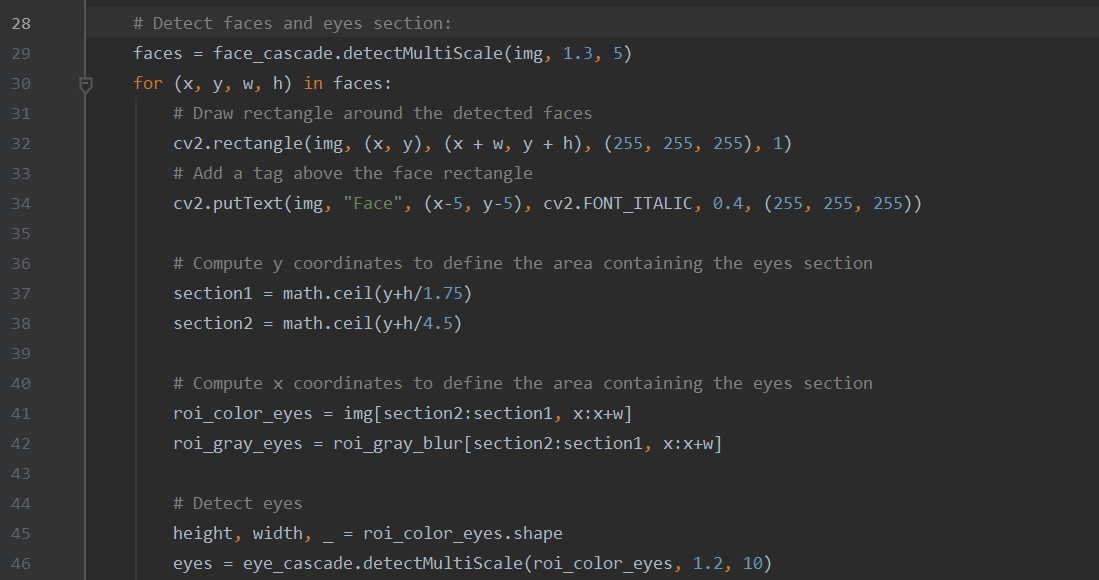
\includegraphics[width=120mm]{img/5/codice_1_3}
	\caption{\fontsize{10px}{0mm}\selectfont Riconoscimento del viso \label{fig:codice_1_3}}
\end{figure}\newline

Una volta terminate le operazioni di processing dell'immagine viene avviata la procedura principale. Essa comincia effettuando una ricerca dei volti all'interno dell'immagine considerata nel dato istante, nel caso positivo, ossia quando vengono riconosciuti dei volti all'interno dell'immagine, l'algoritmo non fa altro che mostrare all'utente un rettangolo attorno ai volti attraverso la finestra mostrata precedentemente.

Durante la fase di progettazione è stato introdotto un concetto, denominato \emph{fascia degli occhi}, che non è altro che l'area del viso all'interno della quale sono presenti gli occhi. Il software, quindi, una volta rilevati dei volti, calcola la fascia degli occhi, che diventerà la nuova region of interest.
All'interno della nuova region of interest verrà avviata una nuova scansione, in particolare, verranno ricercati gli occhi considerando \textit{unicamente} la nuova immagine la cui area corrisponde alla region of interest. Questa scelta migliora le prestazioni sia in termini di computazione, sia in termini di tempo impiegato.\newpage

In questa sezione di codice viene disegnato un rettangolo attorno ad ogni occhio, in particolare indicando precisamente l'occhio sinistro e l'occhio destro.

Arrivati a questo punto, è stata completata la fase iniziale di riconoscimento del viso e degli occhi.
\begin{figure}[h!]
	\centering
	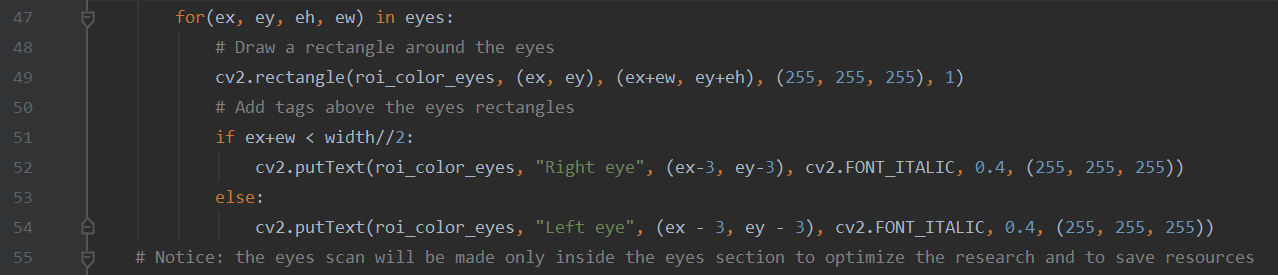
\includegraphics[width=120mm]{img/5/codice_1_4}
	\caption{\fontsize{10px}{0mm}\selectfont Riconoscimento degli occhi \label{fig:codice_1_4}}
\end{figure}

Viene mostrata una finestra contenente la cattura live e le informazioni minimali per l'utilizzo del software.
Grazie alle procedure indicate precedentemente, quando verrà riconosciuto un volto verrà disegnato un rettangolo attorno ad esso, stesso procedimento per gli occhi.

\begin{figure}[h!]
	\centering
	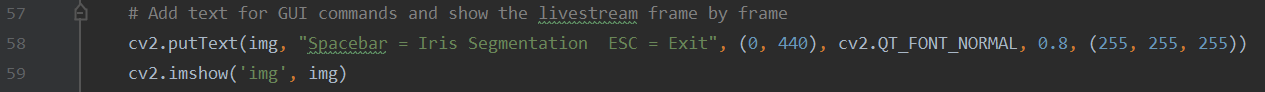
\includegraphics[width=120mm]{img/5/codice_1_5}
	\caption{\fontsize{10px}{0mm}\selectfont Completamento GUI \label{fig:codice_1_5}}
\end{figure}

Arrivati a questo punto, utilizziamo una variabile $$k$$ per catturare gli input dell'utente, in base al tipo di tasto premuto, verrà effettuata un'azione. Quando viene premuto il tasto ESC verrà chiuso il programma.

\begin{figure}[h!]
	\centering
	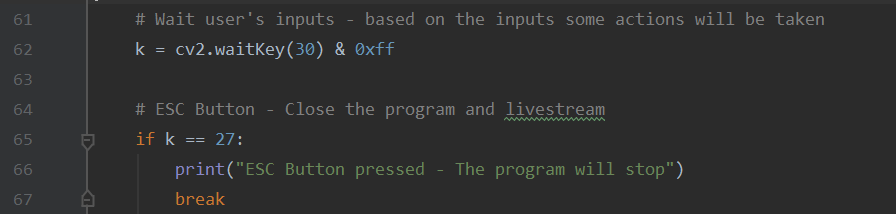
\includegraphics[width=120mm]{img/5/codice_1_6}
	\caption{\fontsize{10px}{0mm}\selectfont Input utente \label{fig:codice_1_6}}
\end{figure}
\newpage
Di seguito è riportata la procedura di segmentazione e codifica dell'iride. Per avviare la procedura l'utente dovrà premere il tasto spacebar, come indicato sulla \ac{GUI}.
Viene utilizzato il metodo \emph{HoughCircles} per permettere l'identificazione della pupilla e della sclera.\footnote{La sclera è la membrana bianca attorno all'occhio}
L'idea è la seguente: una volta individuate le pupille e le sclere, attraverso l'utilizzo di una flag per distinguere l'occhio considerato, viene effettuata la segmentazione delle iridi, in particolare verranno salvate due immagini distinte, una per occhio, contenenti appunto i due occhi. Queste immagini verranno utilizzate in seguito.
Per motivi di design, vengono salvate anche tutte le immagini ottenute durante il processing e durante l'esecuzione del software.
\begin{figure}[h!]
	\centering
	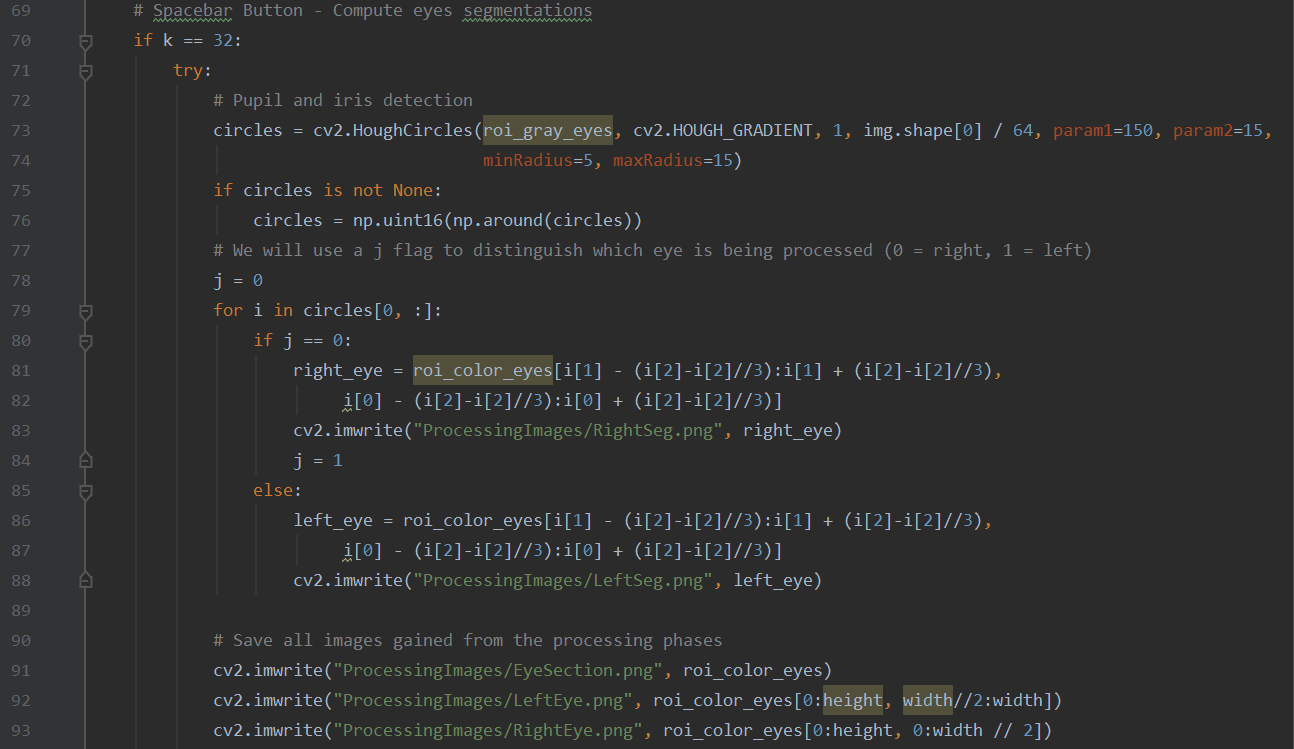
\includegraphics[width=120mm]{img/5/codice_1_7}
	\caption{\fontsize{10px}{0mm}\selectfont Segmentazione dell'iride \label{fig:codice_1_7}}
\end{figure}
L'ultima sezione di codice mostra la fase di chiusura della cattura e il rilascio della webcam, precedute dal metodo segmentation dello script Extract Sector, descritto in seguito. 
\begin{figure}[h!]
	\centering
	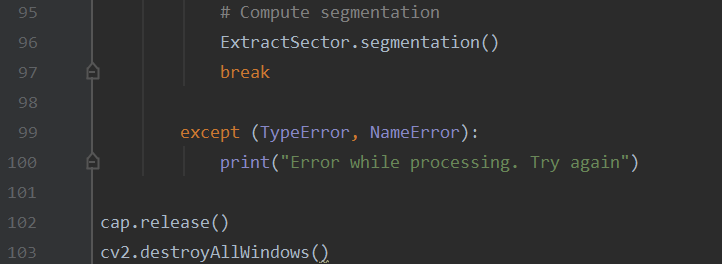
\includegraphics[width=120mm]{img/5/codice_1_8}
	\caption{\fontsize{10px}{0mm}\selectfont Segmentazione dell'iride e Extract Sector \label{fig:codice_1_8}}
\end{figure}\newpage

\subsection{Lo script Extract Sector}
Lo script Extract Sector svolge la fase finale, al fine della quale vengono ottenute le codifiche delle due iridi degli occhi.
In particolare, viene utilizzato \emph{image slicer} per sezionare l'iride considerata, dopodichè viene effettuata la polarizzazione a partire dalle stesse immagini, e infine la codifica.
\begin{figure}[h!]
	\centering
	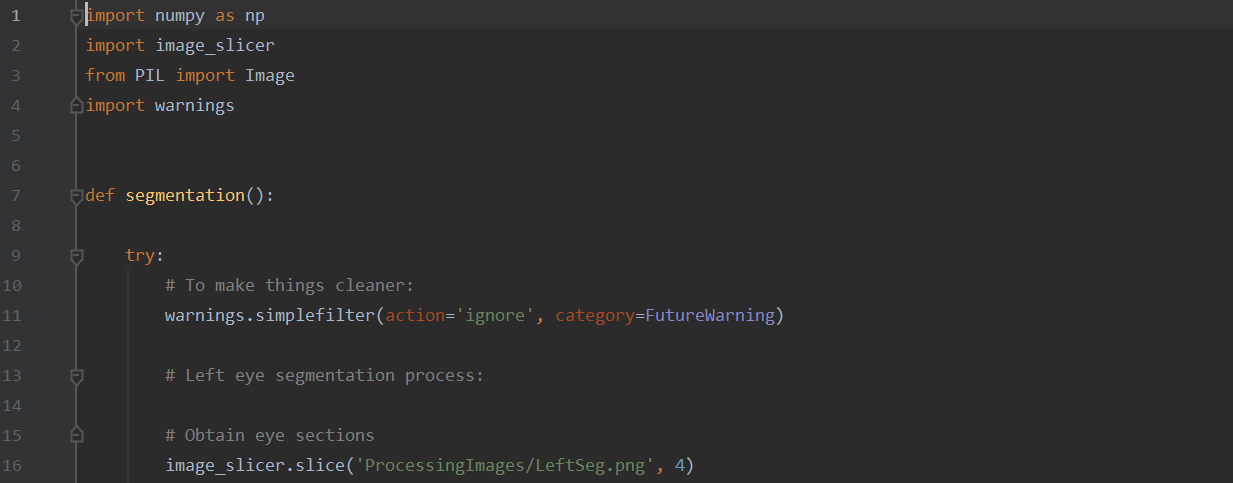
\includegraphics[width=120mm]{img/5/codice_1_9}
	\caption{\fontsize{10px}{0mm}\selectfont Il metodo segmentation \label{fig:codice_1_9}}
\end{figure}
La procedura è identica per entrambi gli occhi. Si inizia ottenendo le quattro sezioni dell'iride e scalandole tutte alla stessa grandezza(in particolare la grandezza della più piccola sezione per evitare di danneggiare l'output finale).
Una volta ottenute le sezioni, si esegue la polarizzazione unendo le immagini in un'unica immagine, sulla quale viene eseguita la codifica.\newpage
\begin{figure}[h!]
	\centering
	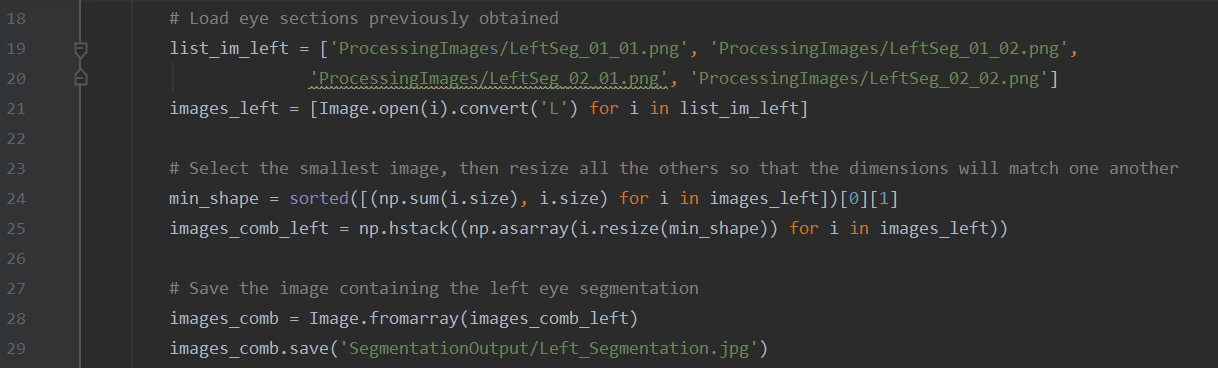
\includegraphics[width=120mm]{img/5/codice_1_10}
	\caption{\fontsize{10px}{0mm}\selectfont Occhio sinistro \label{fig:codice_1_10}}
\end{figure}

\begin{figure}[h!]
	\centering
	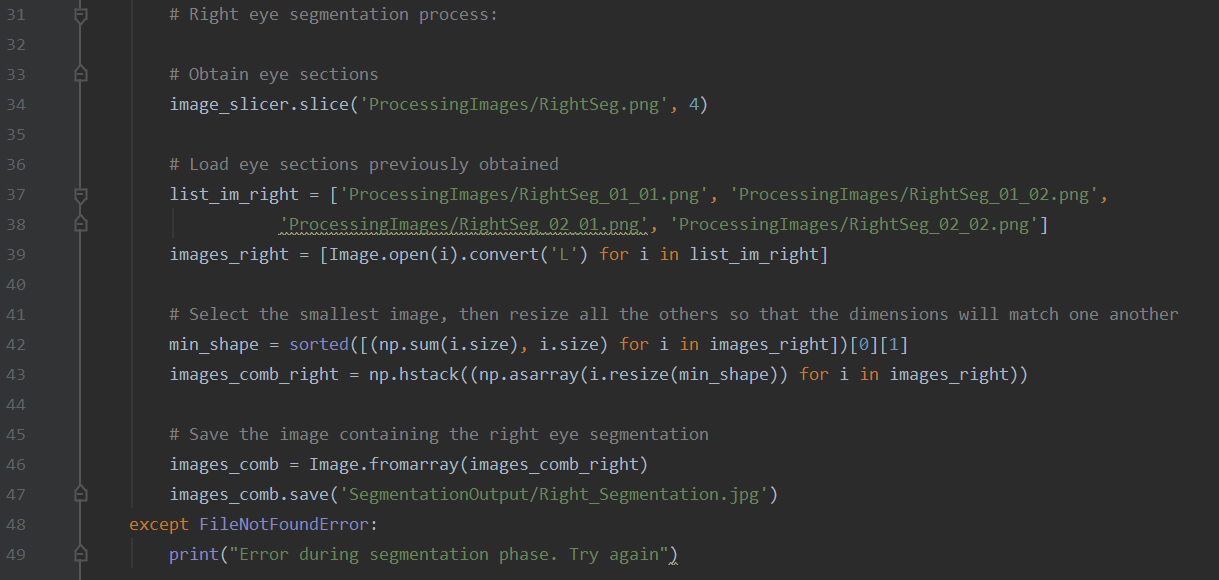
\includegraphics[width=120mm]{img/5/codice_1_11}
	\caption{\fontsize{10px}{0mm}\selectfont Occhio destro \label{fig:codice_1_11}}
\end{figure}
\newpage
		\selectlanguage{italian}
\graphicspath{ {img/6/} }
\chapter{Conclusioni e sviluppi futuri}\label{cap:conclusioni}
\thispagestyle{empty}
\newpage

\section{Conclusioni}
\vspace{8mm}
Il software realizzato ha lo scopo di mostrare il potenziale di un framework di riconoscimento e segmentazione dell'iride in contesti non controllati, utilizzando un dispositivo di utilizzo comune.
Attraverso ulteriori sviluppi tecnologici e attraverso dispositivi ad-hoc per il riconoscimento dell'iride è possibile ottenere un sistema in grado di raggiungere le capacità di un framework basato su riconoscimento delle impronte digitali, possibilmente anche superandole.

\section{Sviluppi futuri}
\vspace{8mm}
Il software utilizza una comune webcam di scarsa qualità, sostituendo l'hardware con un dispositivo ad-hoc è possibile raggiungere risultati molto più rilevanti.
Un possibile miglioramento si basa sull'approccio alla CNN, che però necessita di un dataset molto più ampio e strutturato di quelli attualmente esistenti.

	\backmatter
        \pagestyle{empty}
\fancyhf{}
\cfoot{\thepage}
\pagestyle{fancy}
\chapter{Ringraziamenti}
\vspace{2cm}


Ringrazio il prof. Abate per avermi guidato nella stesura di questo lavoro e per avermi trasmesso la passione 
necessaria al conseguimento di questo traguardo.
Desidero ringraziare il mio tutor, Silvio Barra, che è sempre stato gentile e disponibile nel seguirmi e nel risolvere ogni mio dubbio per tutta la durata del tirocinio interno.
Ringrazio chi ha condiviso con me questi tre anni universitari,in particolare voglio ringraziare Andrea, Mario, Igor e Luca per avermi sostenuto e aiutato nonostante tutto.
Un ringraziamento speciale alla mia famiglia, in particolare a mia madre e mio padre che grazie al supporto costante e ai loro insegnamenti mi hanno permesso di raggiungere questo traguardo e di diventare la persona che sono.

    	\addcontentsline{toc}{chapter}{Bibliografia}
		\printbibliography
\end{document}